\documentclass[11pt,a4paper]{article}

\usepackage{fullpage}
\usepackage{hyperref}
\usepackage{graphicx}
\usepackage{minted}
\usepackage{xcolor}
\usepackage{float}
\usepackage{tabulary}
\usepackage{tabularx}
\usepackage{pdfpages}
\usepackage{subcaption}
\usepackage{adjustbox}
\usepackage{amsfonts}
\usepackage{listings}

\usepackage{fancyhdr}
\pagestyle{fancy}
\fancyhf{}
\usepackage{todonotes}                %% notes from the authors


\renewcommand{\headrulewidth}{0pt}
\renewcommand{\footrulewidth}{0pt}

\fancypagestyle{firstpagefooter} {
	\lfoot{}
	\cfoot{}
	\rfoot{\thepage}
	
}

\lfoot{Name: Florian Morath Legi: 14-931-968}
\rfoot{\thepage}

\begin{document}

\title{Advanced Systems Lab Report\\ \normalsize{Autumn Semester 2018}}
\author{Name: Florian Morath\\Legi: 14-931-968}
\date{
	\vspace{4cm}
	\textbf{Grading} \\
	\vspace{0.5cm}
	\begin{tabular}{|c|c|}
		\hline  \textbf{Section} & \textbf{Points} \\
		\hline  1                &                 \\ 
		\hline  2                &                 \\ 
		\hline  3                &                 \\ 
		\hline  4                &                 \\ 
		\hline  5                &                 \\ 
		\hline  6                &                 \\ 
		\hline  7                &                 \\ 
		\hline \hline Total      &                 \\
		\hline 
	\end{tabular} 
}
\clearpage

\maketitle
\thispagestyle{firstpagefooter}
\newpage

\section{System Overview (75 pts)}

In this section I justify the design choices made for the implementation of the given system description. The goal was to build an efficient and stable system while still keeping it simple to analyze. 

\subsection{Overall architecture}
The main components of the system are the net-thread (\texttt{NetThread.java}), the requests  (\texttt{Request.java}) and the worker threads (\texttt{WorkerThread.java}), which will be explained in more detail in the following subsections. \\

\begin{figure}[!h]
    \centering
	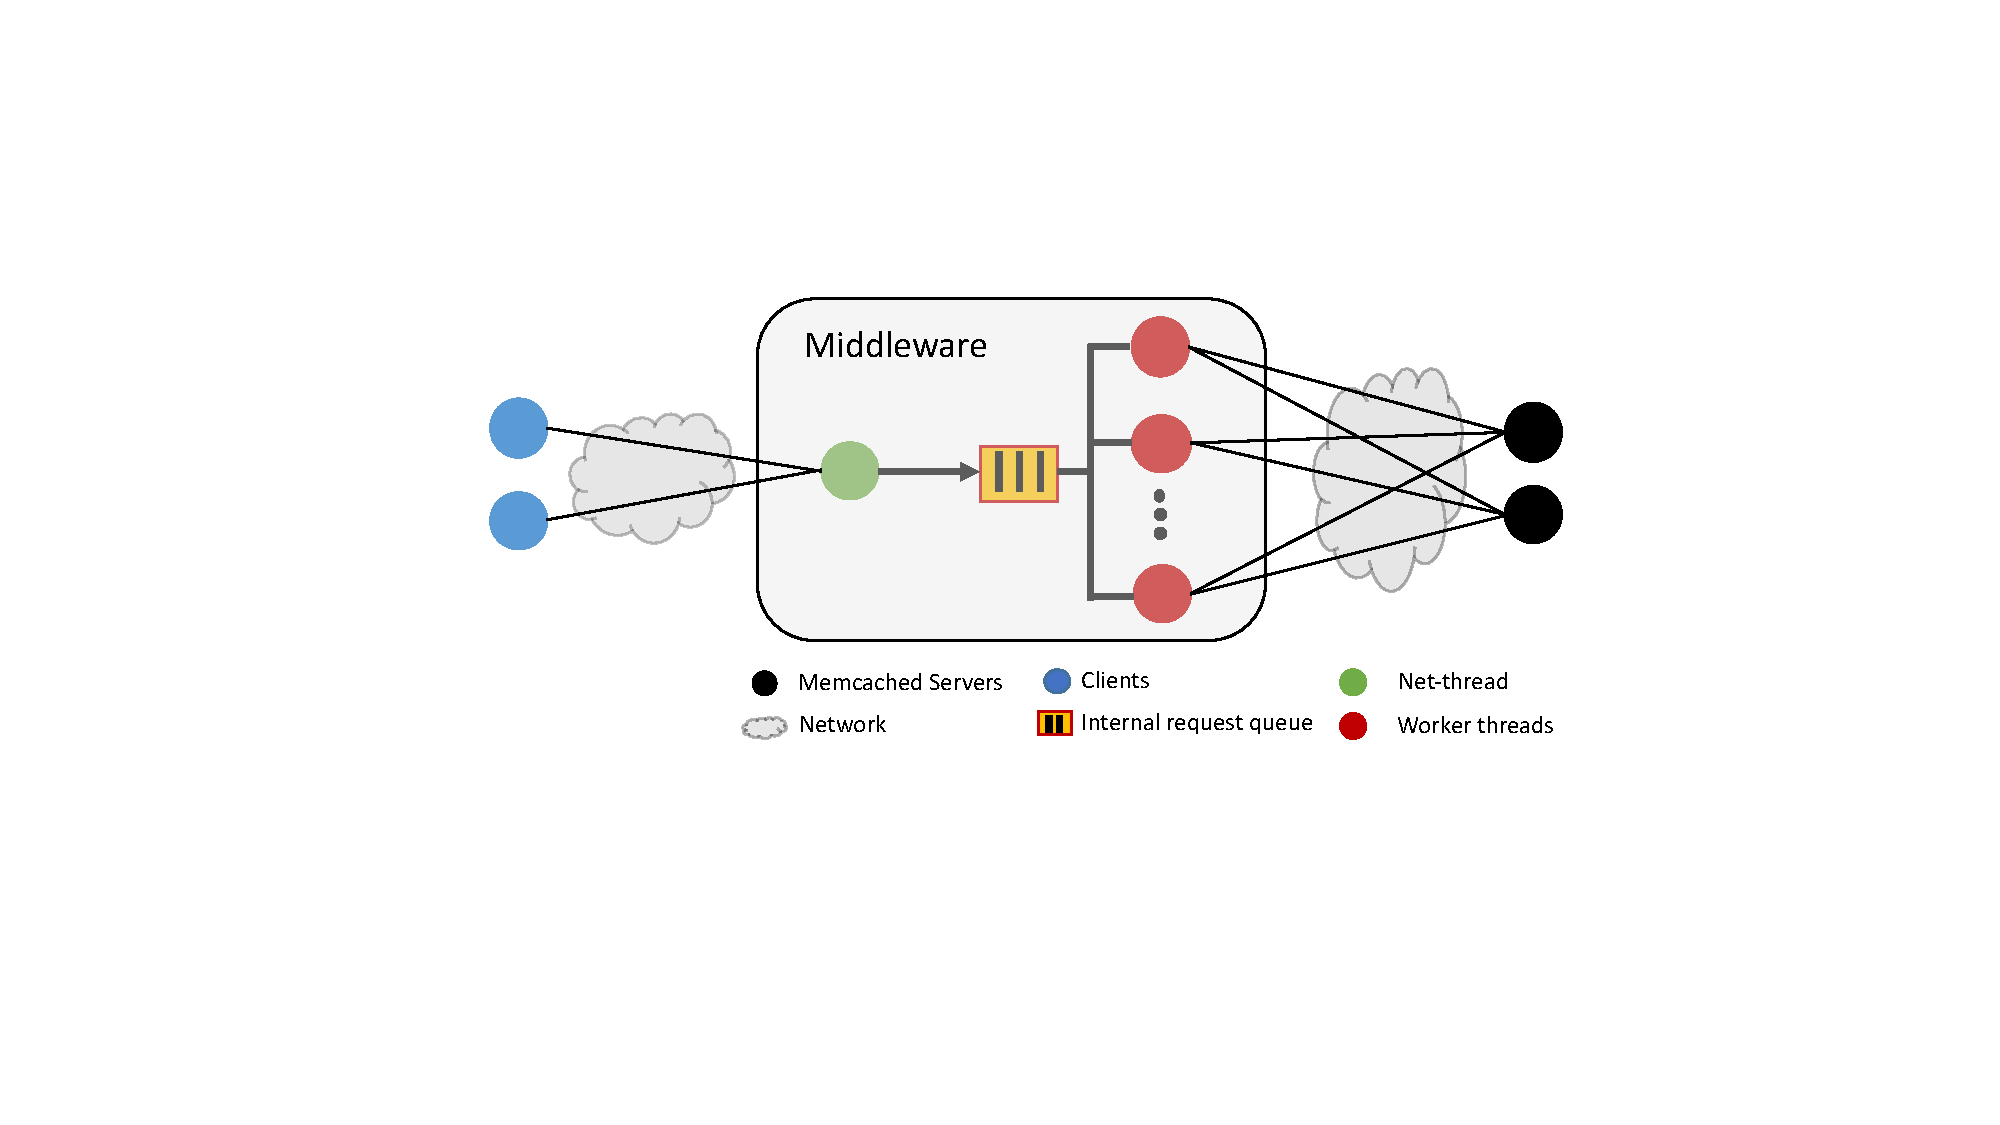
\includegraphics[scale=0.7]{figures/0_SystemOverview/overview_figure.pdf}
	\caption{Interaction between components of the system.}
	\label{overview}
\end{figure}

Figure \ref{overview} gives a simplified overview of the system. First, a client sends a request over a TCP connection to the net-thread. The net-thread reads the message into a buffer, encapsulates it into a \textit{Request} object and puts it into an internal request queue. An available worker thread takes out a request from the queue (if there is one) and processes it depending on its type. The request is sent over a TCP connection to one or multiple servers, after which their response is read into a buffer, then processed and sent back to the client. \\

\texttt{RunMW.java} is the entry point of the system. It parses the command line arguments, such as the addresses of the memcached servers, the address of the net-thread and the number of worker threads in the system. It starts the Middleware by creating an instance of the \textit{Middleware} class, which then starts the worker threads and the net-thread. 

\subsection{Net-Thread}
The \texttt{NetThread} class extends the \textit{Thread}\footnote{\url{https://docs.oracle.com/javase/8/docs/api/java/lang/Thread.html}} class. 
The net-thread basically does two things: It establishes client connections and puts received requests into a queue. \\

% client connections
A \textit{Selector}\footnote{\url{https://docs.oracle.com/javase/8/docs/api/java/nio/channels/Selector.html}} is used to handle multiple connections with a single thread. A selector can monitor multiple connections for certain I/O events and notify the net-thread when they occur. At first, the net-thread creates a server socket channel which it binds to its address. This channel's sole purpose is to accept new connections from clients. It is registered with the selector for "accept events", i.e. the selector monitors incoming connections on the server socket channel. When this event happens, the net-thread gets notified by the selector and creates a new socket channel for the connection to the client. New socket channels are registered with the selector for "read events", i.e. the selector monitors when data from the clients is ready to be read from. Again, when this event occurs, the net-thread gets notified and reads the data. Note that the net-thread has to call the blocking \textit{select()} method on the selector to be notified for those events.\\
% why Selector, advantages, consequences, non-blocking I/O
This design allows the net-thread to monitor multiple channels for I/O events at the same time. It also enables non-blocking I/O between the clients and the net-thread without having the net-thread to constantly poll the medium and wasting CPU resources. \\

% buffer
We want to minimize the number of times we allocate \textit{ByteBuffer}\footnote{\url{https://docs.oracle.com/javase/8/docs/api/java/nio/ByteBuffer.html}} objects and reuse them as often as possible to minimize both data copy operations and memory allocation on the heap. The net-thread only needs to allocate one buffer per client connection because we have a closed system, i.e. clients wait for a response before sending the next request. Therefore, before sending a response to the client, we just clear the buffer associated with this client connection such that it can be reused again for a new request from this client. Since we have a fixed number of clients, the number of buffer allocations by the net-thread is also fixed and does not grow with the number of request. \\
We associate a buffer with each client connection using the \textit{SelectionKey}\footnote{\url{https://docs.oracle.com/javase/8/docs/api/java/nio/channels/SelectionKey.html}} object. A selection key is created whenever we register a channel with a selector. Most importantly, it contains the channel for which the key was created and an attachment where we can store any object. We use this attachment to associate a buffer with each client connection. \\

% request enqueueing
Whenever a full request has been read into a byte buffer by the net-thread, it encapsulates it in a \textit{Request} object and puts it into the internal request queue. More details about the \textit{Request} class and the queue will be given in the next subsection. 

\subsection{Requests}
% LinkedBlockingQueue (why, advantages -> unbounded?, thread safe, take out is blocking, add non-blocking)
There are several reasons why we have chosen a \textit{LinkedBlockingQueue}\footnote{\url{https://docs.oracle.com/javase/8/docs/api/java/util/concurrent/LinkedBlockingQueue.html}} to enqueue and dequeue requests. First of all, we use a blocking queue because the \textit{take()} operation should block until an element becomes available, which is more efficient (in terms of CPU usage) than constantly polling the queue and checking if an element is in there. \\
We use the linked implementation (in contrast to the array implementation) because of the following reasons: We have constant time for the take() and put() operation because doubly-linked nodes are used as an internal data structure. There is a separate lock for the head and the tail, which may result in better throughput because we can add and remove elements simultaneously. The default capacity is \mintinline{java}{Integer.MAX_VALUE}, which can be considered unbounded. That's good because we don't know how many requests may be in the queue and also we don't have to allocate space for requests a priori as for the \textit{ArrayBlockingQueue}. \\
However, there is a disadvantage in choosing the linked blocking queue, namely that the performance may be more variable than with an array blocking queue because of the dynamic allocation of nodes during usage and the more complicated data structure with doubly-linked nodes. \\

% explain fields
Requests from clients are encapsulated in \textit{Request} objects. The \textit{Request} class contains the following fields: 
\begin{itemize}
    \item \textbf{buffer}: The byte buffer into which the request from the client was written into.
    \item \textbf{key}: A selection key which contains the channel over which the request was sent to the net-thread. This channel is used by the worker threads to be able to send the response back to the correct client. 
    \item \textbf{type}: The type of the request which is either a Set, a Get (includes Multiget) or an Invalid request. 
    \item \textbf{instrumentation fields}: See subsection \ref{sub:instr}.
\end{itemize}
% explain parseMethod
The constructor of the \textit{Request} class calls a method \textit{parseRequest()}, which first checks if there is an end of line string \texttt{\textbackslash r\textbackslash n} at the last two written bytes of the byte buffer. If there is none, the request is considered Invalid. Then the type of the request is determined based on the first three chars of the request which should be either 'get' or 'set'. Note that the distinction between Multiget and Get requests is not done at this point in order to avoid code duplication and keeping the code simple. 

\subsection{Worker Threads}
% role of worker threads, what do they do
The \texttt{WorkerThread} class extends the \textit{Thread}\footnote{\url{https://docs.oracle.com/javase/8/docs/api/java/lang/Thread.html}} class. 
The role of the worker threads is basically to establish connections to the memcached servers and to process the requests that the net-thread added to the internal request queue. \\

% First: memcached server connections (blocking)
The first thing a worker thread does is to establish a permanent connection to each memcached server. The addresses of those servers are passed as an argument to the middleware at start-up. A worker thread opens a socket channel for each server and connects it to the server. The socket channels are stored in an array list, in order to be able to access them later on. The channels are configured to be blocking to keep the code simple and to not waste CPU resources while polling until a whole response has been read from a server. However, it also has disadvantages like failure during blocking calls leading to unresponsiveness and scalability issues if we have a lot of open connections, which in our case we don't have because we can have at maximum three servers. \\

% write about buffers (efficient allocation and reusability of responseBuffer)
For the buffer allocations, once again, we want to use as few allocations as possible and reuse them. This is achieved by having each worker thread allocating one buffer and referencing it with a field. This buffer is used to write the response from the servers into. If a request is done being processed, the buffer can be cleared in order to be reused again. Note that because of the sharded mode we actually allocate another buffer to make the reassembly of the responses easier, which will be explained later in more detail. But still the number of buffers doesn't grow with the number of requests and stays proportional to the number of worker threads.\\

The main loop of the worker thread consists of taking out a request from the queue (this is a blocking operation), processing it depending on its type and when finished taking out another one and so forth. \\
If the type of the request is \mintinline{java}{SET} then it will call \textit{handleSetRequest()}, if it is \mintinline{java}{GET} then it will call \textit{handleGetReuquest()} and if it is \mintinline{java}{INVALID}, it will send the error message "\mintinline{java}{ERROR}\texttt{\textbackslash r\textbackslash n}" to the client having sent the request.

% two subsubsections: different kind of requests (set and get request): explain each execution path in detail
\subsubsection{Handle a Set Request}
For a Set request, the worker thread sends it to each server and then waits for a response of all of them. If one or multiple servers respond with an error message, one of them is forwarded to the client. If no error occurred, one of the success messages is forwarded to the client. \\
This is implemented as follows: The buffer contained in the \textit{Request} object is sent sequentially to each server by iterating over the socket channels. After that, we go over the socket channels again and for each socket channel we write the response into our buffer and check the content in order to find out if the Set request was successfully executed on the server. If it was not, the error message is added to an array list. Note that we always read from a channel until we get an end of line string, which denotes that a full response has been read. And also note that the buffer is cleared before writing into it, such that we can reuse it and not have to allocate a new one for each response. After having processed all responses, if there occurred an error, we just forward the first error message to the client and otherwise the last success message is forwarded to the client because it is still contained in the buffer. 

\subsubsection{Handle a Get Request}
For the \textbf{non-sharded mode}, we just forward the Get request (includes Multiget requests) to one server, which is chosen based on a round-robin scheme, and the response from the server is forwarded to the client. We don't have to inspect the response because independently of success or error, it can always be forwarded to the client. \\
The round-robin scheme works by having a private field \textit{'lastServerIndex'} in each worker thread,  which identifies the last server used by this worker thread for a Get request. Whenever a worker thread sends a (non-sharded) Get request, it executes the following code to retrieve the socket channel it uses to write the request to. Note that \textit{'socketChannels'} is an array list containing all established socket channels to the servers.   
\begin{minted}[frame=single]{java} 
    lastServerIndex = (lastServerIndex + 1) % socketChannels.size();
    SocketChannel socketChannel = socketChannels.get(lastServerIndex);
\end{minted}
 The empirical evaluation of the load balancing and the justification of this design choice is given in subsection \ref{sub:lb}. \\
  
For the \textbf{sharded mode}, a Multiget request has to be evenly split into a set of smaller Multiget requests, one for each server. Note that if there are fewer keys in the request than servers, we need to load balance them such that whenever this case occurs, not always the same servers are hit. To simplify the explanation, we ignore this case for the moment. \\
First we extract the keys from the request and put them into the '\textit{keys'} array. There can be between 1 and 10 keys. Each server is identified with an index which corresponds to the position of its socket channel in the \textit{'socketChannels'} array. We then need to figure out the number of keys each server should handle such that they are evenly distributed and sum up to the total number of keys in the \textit{'keys'} array. We do this based on the index which identifies a server: 
\begin{minted}[frame=single]{java}
    public static int getKeyCount(int index, int numKeys, int serverCount) {
        int keyCount = 0;
        for (int i = index; i < numKeys; i += serverCount) {
            keyCount++;
        }
        return keyCount;
    }
\end{minted}
\textit{getKeyCount()} is a method that returns the number of keys for which a server with a specific index is responsible for. \textit{'numKeys'} is the total number of keys in the request and \textit{'serverCount'} is the total number of servers. It works by counting how many times we can add the 'serverCount' to the index until we exceed the 'numKey'. For example if we have 3 servers and 7 keys, index 0 gets 3 keys, index 1 gets 2 keys and index 2 gets 2 keys which sums up to 7 keys and is evenly distributed. \\
For each server we do the following: Construct the Get request based on its \textit{'getKeyCount()'}. The keys are retrieved from the \textit{'keys'} array in-order, i.e. the server with index 0 retrieves the first n elements, then the server with index 1 retrieves the next m elements and so on. \\
After all Get requests have been sent, we retrieve the responses from the servers in the same order as we have sent the requests, which simplifies the reassembly of the responses. The responses are reassembled into one response in a separate buffer for simplicity. In case of an error message, an error flag is raised and in the end '\mintinline{java}{ERROR}\texttt{\textbackslash r\textbackslash n}' is sent to the client instead of the reassembled response. \\
What is left to explain is how we handle the case with fewer keys than servers. Since we don't want to always hit the first n servers in the \textit{'socketChannels'} array, where n is the number of keys, we apply the same round-robin scheme as in the non-sharded mode. But now we need to keep track of which servers we queried and in which order we did it, in order to be able to reassemble the responses in the correct order. For this we use an array called \textit{'usedServers'}. The value of \textit{'usedServers'} at position i tells if we did send a request to a server at iteration i, and if yes to which we did send one. 

\subsection{Load Balancing} \label{sub:lb}
% design choice
To denote the last server used in the round-robin scheme, we have chosen to use a private field \textit{'lastServerIndex'} in each worker thread instead of a global variable because it avoids having to synchronize access on it. Having all worker threads access the same variable for every Get request concurrently would lead to blocking behavior, which degrades the performance. 

% empirical evaluation -> show plot
We did an empirical evaluation to show that on average all memcached servers are subject to the same load. The experiment was run on the cluster with 1 client, 4 worker threads and 3 memcached servers with Get requests only. Each worker thread printed how many times it hit each of the servers:
\begin{lstlisting}[basicstyle=\tiny]                
[Thread-2] ch.ethz.asl.WorkerThread: [0=16208, 1=16208, 2=16208] 
[Thread-4] ch.ethz.asl.WorkerThread: [0=15208, 1=15209, 2=15208] 
[Thread-5] ch.ethz.asl.WorkerThread: [0=15753, 1=15754, 2=15753] 
[Thread-3] ch.ethz.asl.WorkerThread: [0=16307, 1=16308, 2=16308] 
\end{lstlisting}
Server 0 was hit 63'476 times, server 1 was hit 63'479 times and server 2 was hit 63'477 times which shows that the load is distributed equally among the servers.

\subsection{Instrumentation} \label{sub:instr}
The following timestamps are collected during the lifetime of a request:
\begin{itemize}
    \item \textbf{timeFirstByte}: Time at which the first byte of the request is read by the net-thread.
    \item \textbf{timeEnqueued}: Time at which the request is enqueued into the internal request queue by the net-thread. 
    \item \textbf{timeDequeued}: Time at which a worker thread dequeues the request from the internal request queue.
    \item \textbf{timeMemcachedSent}: Time immediately before the worker thread sends the (first) request to a memcached server. 
    \item \textbf{timeMemcachedReceived}: Time immediately after the (last) response of a memcached server was read by the worker thread. 
    \item \textbf{timeCompleted}: Time at which the worker thread sends the response back to the client. 
\end{itemize}
All those timestamps, the queue length after the request is dequeued and the request type is stored in the \textit{Request} object itself. After the request is completed, the worker calls the method \textit{writeLogLine()} on it, which writes the instrumentation data to a csv-file. Note that we use \textit{Log4j} for logging, which is configured to not immediately flush on each \textit{log()} invocation, but buffers the logs until its capacity of 8'192 bytes is reached. We compared experiments with and without logging in order to check that logging does not affect the performance of the middleware. 

Aggregation of log-files is outsourced to python scripts which run after the experiments are finished. A more detailed explanation of the postprocessing can be found in the \textit{README} files of the repository.

\section{Baseline without Middleware (75 pts)}
% Intro

% Purpose
The purpose of this section is to study the performance characteristics of the \textit{memtier} clients and \textit{memcached} servers. \\
% Experimental setup
The experimental setup is as follows: We let each experiment run for 80s and each experiment is repeated 3 times. The standard deviation of a specific metric is computed over those repetitions and shown as red error bars in the plots. Note that if the standard deviation is very small, one might not be able to see the red error bars in the plots. Throughput and response time are based on the output of \textit{memtier}, whereas other metrics like the CPU utilization are based on the output of \textit{dstat}. 

\subsection{One Server}
% setup description
In this setup we have 3 memtier instances (each installed on a single VM) connected to a single memcached instance. The overview of the experiment parameters is given in the following table:
\begin{center}
	\scriptsize{
		\begin{tabular}{|l|c|}
			\hline Number of servers                & 1                        \\ 
			\hline Number of client machines        & 3                        \\ 
			\hline Instances of memtier per machine & 1                        \\ 
			\hline Threads per memtier instance     & 2                        \\
			\hline Virtual clients per thread       & \{2,4,8,16,24,32,40\} \\ 
			\hline Workload                         & Write-only and Read-only \\
			\hline Repetitions                      & 3                        \\ 
			\hline 
		\end{tabular}
	} 
\end{center}

% plots
\begin{figure}[H]
   \begin{minipage}{0.48\textwidth}
     \centering
     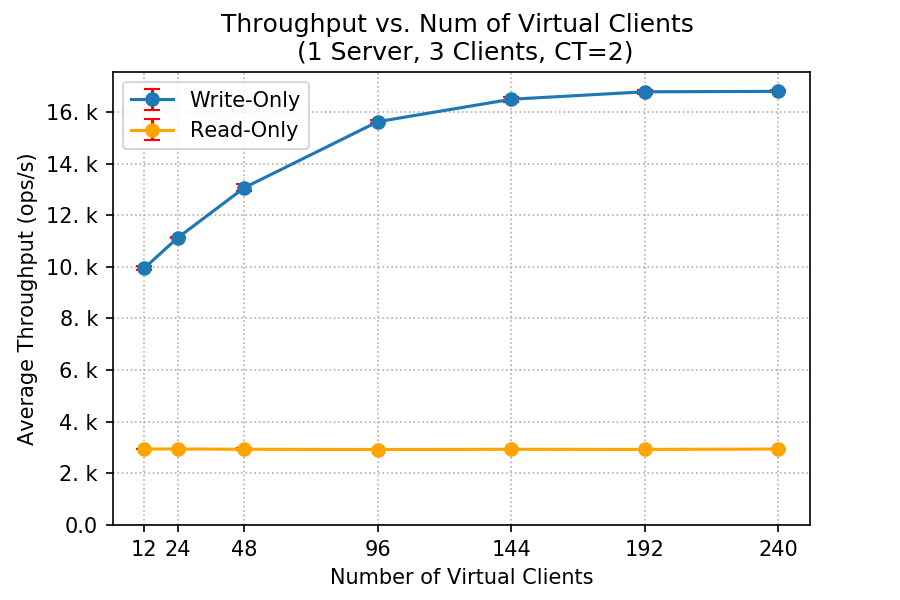
\includegraphics[width=1\linewidth]{figures/1_BaselineWithoutMW/one_server/one_server_mem_tp_2018-10-21_20h12.png}
     \caption{Average throughput.}\label{one_server_tp}
   \end{minipage}\hfill
   \begin{minipage}{0.48\textwidth}
     \centering
     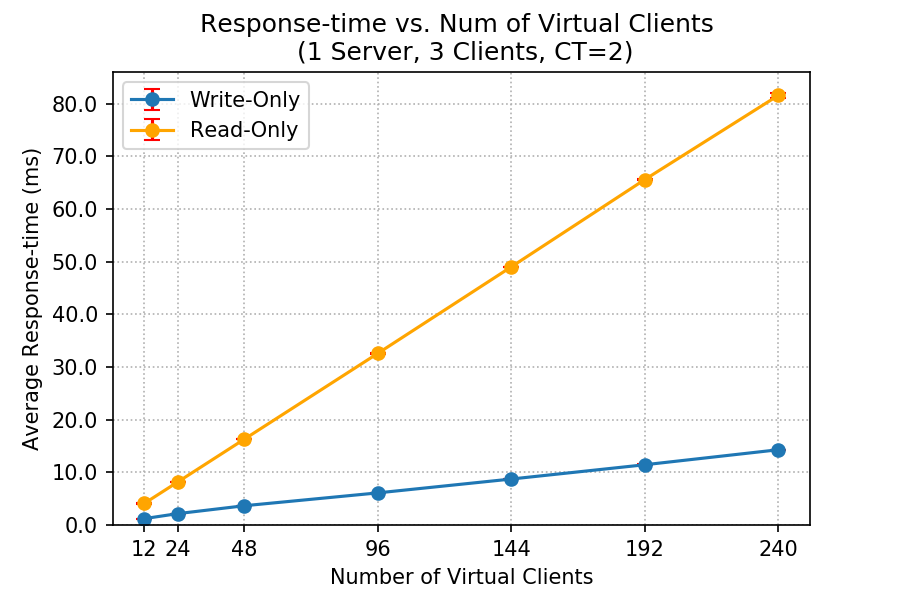
\includegraphics[width=1\linewidth]{figures/1_BaselineWithoutMW/one_server/one_server_mem_rt_2018-10-21_20h12.png}
     \caption{Average response time.}\label{one_server_rt}
   \end{minipage}
\end{figure}
The throughput as a function of virtual clients for read-only and write-only workloads is given in Figure \ref{one_server_tp}, whereas the response time as function of virtual clients for read-only and write-only workloads is given in Figure \ref{one_server_rt}. 

% explanation
% interactive law
The interactive response time law relates throughput and response time in a closed system. It states that $R=N/X-Z$ with response time $R$, throughput $X$, think time $Z$ and $N$ number of clients. $Z$ is often assumed to be zero. The interactive law was checked and holds. Note that for the remaining chapters, the interactive law will be checked for all throughput and response time plots, and unless explicitly stated otherwise, it can be assumed to hold. 

% write throughput: where does memcached saturate, why (what’s the bottleneck)? 
% -> show CPU utilisation plot (dstat) (at 100 percent utilisation) 
If we look at the throughput in Figure \ref{one_server_tp}, we can see that for write-only workloads the system saturates at around $144$ virtual clients because after that the throughput flattens. The CPU utilization plot of the memcached server, which can be seen in Figure \ref{cpu_utilization_one_server}, shows that the CPU is the bottleneck here because it almost reaches full utilization at around the saturation point. 

\begin{figure}[H]
    \begin{minipage}{0.48\textwidth}
        \centering
	    \includegraphics[scale=0.48]{figures/1_BaselineWithoutMW/one_server/dstat_server_cpu_ratio_1:0_2018-10-21_20h12.png}
	    \caption{CPU utilization of a server VM during write-only workload.}
	    \label{cpu_utilization_one_server}
    \end{minipage}\hfill
    \begin{minipage}{0.48\textwidth}
        \centering
	    \includegraphics[scale=0.48]{figures/1_BaselineWithoutMW/one_server/dstat_server_netsend_ratio_0:1_2018-10-21_20h12.png}
	    \caption{Outbound network activity of a server VM during read-only workload.}
	    \label{outbound_net_activity_one_server}
    \end{minipage}
\end{figure}

% read throughput: where does memcached saturate, why (what’s the bottleneck)? 
% network bandwidth, figure out network bandwidth with iperf and then actually used bandwidth with dstat.
% (server upload bandwidth at 12Mbps which is max with  iperf) 
The throughput for read-only workloads stays at the same level during the whole experiment. This indicates that the network bandwidth might be a bottleneck here. In order to confirm this, we first we need to check the maximum outbound network bandwidths for clients and servers. This is done with \textit{iperf}, the results can be seen in the following table: 

\begin{center}
	\begin{tabular}{|l|c|}
	    \hline    & Maximum outbound network bandwidth          \\
		\hline Server VM  & 12.6 MB/s           \\ 
		\hline Client VM & 25 MB/s           \\ 
		\hline 
	\end{tabular}
\end{center}

Now that we know the maximum outbound network bandwidth, we can check the actually used network bandwidth. Figure \ref{outbound_net_activity_one_server} shows that indeed the network activity of memcached server is at its limit and thus the bottleneck of read-only workloads. That the network send activity does not stay perfectly at 12.6 MBps I attribute to noise in the cluster. We can compute the maximal throughput based on the maximal bandwidth of the server to support our claim: A single response from the server is around 4kB because it contains a single value corresponding to a key. Thus if we divide 12.6 MBps by 4kB, we get around 3k requests per second which is exactly what we measured. Saturation is already reached for the lowest number of clients which is why we don't observe under-saturation. 

% response time
Finally we look at the response times in Figure \ref{one_server_rt}. We observe that for read-only workloads the response-time grows faster than for write-only workloads. This makes sense because of the lower throughput for the read-only workloads. \\

\subsection{Two Servers}

% setup description
In this setup we have 2 memtier instances (both run on the same VM), each of which is connected to a single memcached instance. Each memcached instance is installed on a separate VM, i.e. we have two server VMs in total. The overview of the experiment parameters is given in the following table: 
\begin{center}
	\scriptsize{
		\begin{tabular}{|l|c|}
			\hline Number of servers                & 2                        \\ 
			\hline Number of client machines        & 1                        \\ 
			\hline Instances of memtier per machine & 2                        \\ 
			\hline Threads per memtier instance     & 1                        \\
			\hline Virtual clients per thread       & \{1,4,8,16,24,32,40\}        \\ 
			\hline Workload                         & Write-only and Read-only \\
			\hline Repetitions                      & 3              \\ 
			\hline 
		\end{tabular}
	} 
\end{center}

% plots
The throughput as a function of virtual clients for read-only and write-only workloads is shown in Figure \ref{two_server_tp}, whereas the response time as function of virtual clients for read-only and write-only workloads is shown in Figure \ref{two_server_rt}. 
% data: [2018-12-06_10h49]
\begin{figure}[H] % [!htb]
   \begin{minipage}{0.48\textwidth}
     \centering
     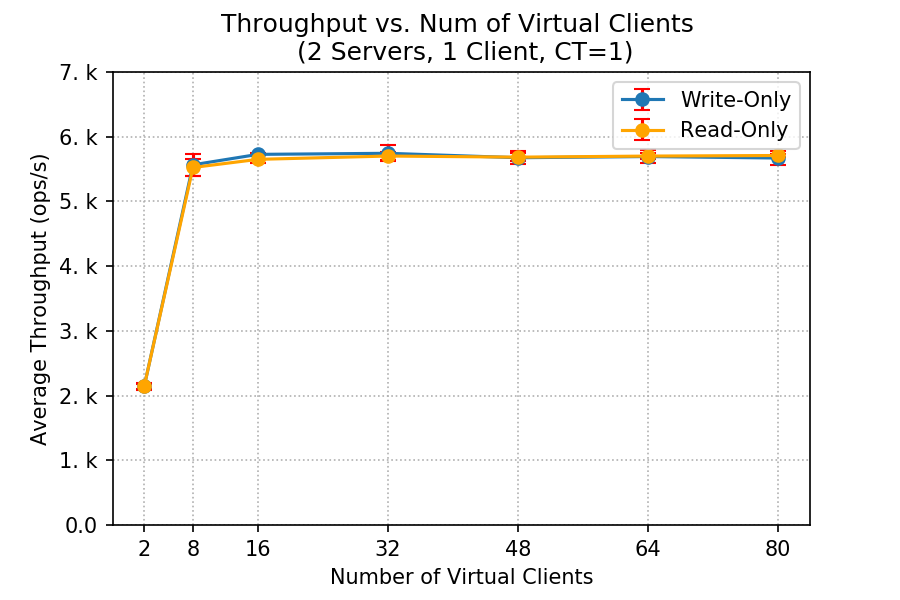
\includegraphics[width=1\linewidth]{figures/1_BaselineWithoutMW/two_servers/two_servers_mem_tp_2018-12-06_10h49.png}
     \caption{Average throughput.}\label{two_server_tp}
   \end{minipage}\hfill
   \begin{minipage}{0.48\textwidth}
     \centering
     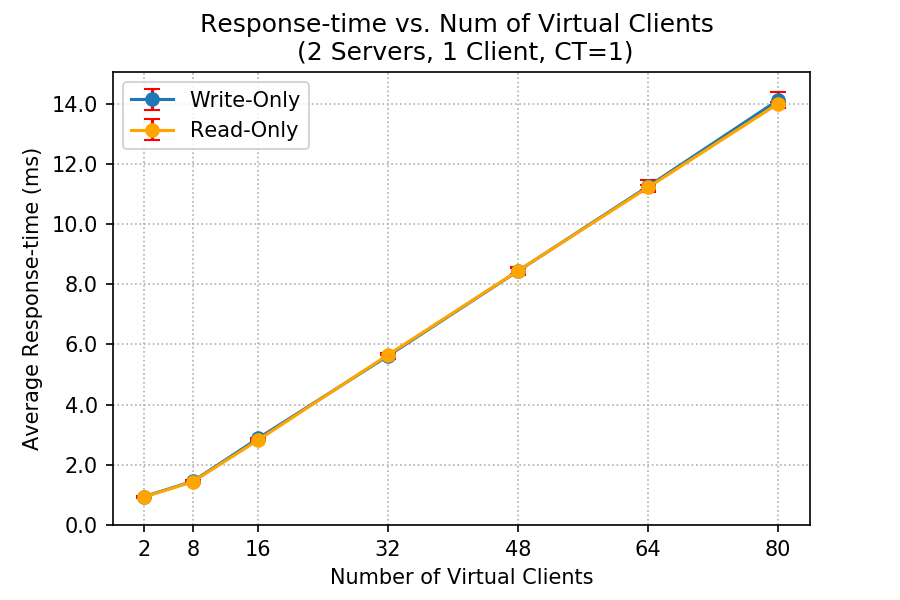
\includegraphics[width=1\linewidth]{figures/1_BaselineWithoutMW/two_servers/two_servers_mem_rt_2018-12-06_10h49.png}
     \caption{Average response time.}\label{two_server_rt}
   \end{minipage}
\end{figure}

% explanation
% interactive law
First of all the interactive law was checked and holds. 
% write throughput: where does memcached saturate, why (what’s the bottleneck)? 
% -> show outbound bandwidth at memtier (at 23MBps)
For write-only workloads the system  already saturates at $8$ virtual clients because from this point on, the throughput flattens and the response time starts increasing significantly, as it can be seen in Figures \ref{two_server_tp} and \ref{two_server_rt}. The bottleneck here is the outbound network bandwidth of the client VM. This can be seen in Figure \ref{outbound_client_net_activity_two_servers} which shows that the maximum bandwidth of $25$ MB/s (checked with \textit{iperf}) for the client VM is reached. The network send activity not being perfectly at $25$ MBps I attribute to noise on the cluster.

% data: [2018-12-06_10h49]
\begin{figure}[H]
	\begin{minipage}{0.48\textwidth}
	    \centering
	    \includegraphics[scale=0.48]{figures/1_BaselineWithoutMW/two_servers/dstat_client_netsend_ratio_1:0_2018-12-06_10h49}
	    \caption{Outbound network activity of the client VM.}
	    \label{outbound_client_net_activity_two_servers}
   \end{minipage}\hfill
   \begin{minipage}{0.48\textwidth}
        \centering
	    \includegraphics[scale=0.48]{figures/1_BaselineWithoutMW/two_servers/dstat_server_netsend_ratio_0:1_2018-12-06_10h49.png}
	    \caption{Outbound network activity of a server VM.}
	    \label{outbound_server_net_activity_two_servers}
   \end{minipage}
\end{figure}

%read throughput: where does throughput reach saturation? bottleneck?
%->outbound bandwidth at server (12MBps)
For read-only workloads the system also saturates at $8$ virtual client for the same reasons, as can be seen in Figures \ref{two_server_tp} and \ref{two_server_rt}. The bottleneck here is also the outbound network bandwidth, but now of the server VMs and not the client VM. This can be seen in Figure \ref{outbound_server_net_activity_two_servers}, which shows that the maximum bandwidth of $12.6$ MB/s (checked with \textit{iperf}) for the server VM is reached at $8$ virtual clients, which is exactly the saturation point of the read-only workload. 

% general remark: set size resp. get response size -> bottleneck
Note that those results also make sense because for the read-only workloads the responses contain $4$ kB values, which mainly affect the outbound bandwidth at the server, whereas the requests just contain the keys which require a few bytes. On the other hand, for the write-only workloads we have the opposite case, i.e. the requests contain the $4$ kB values, which leads to an outbound bandwidth problem at the clients and the responses just contain a status code of a few bytes. 

\subsection{Summary}

\begin{center}
	{Maximum throughput of different VMs.}
	\begin{tabular}{|l|p{2.5cm}|p{2.5cm}|p{4cm}|}
		\hline                        & Read-only workload & Write-only workload & Configuration giving maximum throughput \\ 
		\hline One memcached server   &  2'924 reqs/s & 15'624 reqs/s & 12 clients for read-only, 96 clients for write-only        \\ 
		\hline One load generating VM & 5'897 reqs/s & 5'976 reqs/s   & 8 clients for read-only and write-only           \\ 
		\hline 
	\end{tabular}
\end{center}
The table above shows the maximum throughput for both experiments. Note that when determining the maximum throughput of the system, we take the response time and how it is affected by the increase in load into consideration. For the one server case and write-only workload, going from 96 to 144 clients increases the throughput by $5.6 \%$ while increasing the response time by $30 \%$, which is why we chose the 96 client configuration. For the one server case and read-only workload, we choose the lowest number of clients because the throughput remains the same while the response time increases with more clients. For the two server case and write-only workload, going from 8 to 16 clients increases the throughput by $2.8 \%$, while increasing the response time by $50 \%$ and similar numbers for the read-only workload. 

% one server
For the one server experiment, we tested the limits of a single server. For write-only workloads the bottleneck is its CPU and for read-only workloads the bottleneck is its outbound network bandwidth, which is plausible because for the writes it has to process a lot of big requests, and for the reads it has to send back big responses. The reason that reads have a much smaller throughput than the writes is that the server only has a $12$ MBps outbound network bandwidth, which is a much more limiting factor than the CPU for the writes. 

% two server
For the two server experiment, we tested the limits of a single client. For both kind of workloads the bottleneck is the network bandwidth and the throughput is very similar, which I guess is just a coincidence based on the maximal outbound network bandwidth of the client and the server VM. 

% Comparison
Comparing the read-only throughput of the experiments, we observe that doubling the number of servers also roughly doubles the read-only throughput on average. This is because in the one server case we did not provide enough server bandwidth resources. 
Comparing the write-only throughput of the experiments, we observe that the one server case has roughly $2-3$ times the throughput of the two server case. This is because in the two server case we did not provide enough client bandwidth resources. 

% Take-away messages about behavior of clients and servers
The conclusion is that the server and client resources need to be carefully selected for the performance analysis of the middleware. If we want the observe the bottlenecks of the middleware, we need to provide enough resources such that we are not limited for example by the network bandwidth or CPU of the server or client VMs. 

\section{Baseline with Middleware (90 pts)} \label{section:BaselineWithMW}
%% Intro

% Purpose
In this section we put either one or two middlewares between the \textit{memtier} clients and the \textit{memcached} servers. The purpose of this is to study the performance effects of our middleware. \\
% Experimental setup
The experimental setup is as follows: We let each experiment run for 80s and each experiment is repeated 3 times. The first and last 10 seconds of an experiment are considered to be unstable and are thus ignored. The standard deviation of a specific metric is computed over those repetitions and shown as error bars in the plots. From the outputs of the middleware we compute average queue length, a detailed breakdown of the response time and throughput of the middleware. In addition, the throughput and overall response time is computed from the outputs of the \textit{memtier} instances. Different kinds of resource usage statistics are computed with \textit{dstat}.

\subsection{One Middleware} \label{sec:baselineWithMWOne}
% setup description
In this setup we connect three load generator machines to a single middleware and use one memcached server. The overview of the experiment parameters is given in the following table:
\begin{center}
	\scriptsize{
		\begin{tabular}{|l|c|}
			\hline Number of servers                & 1                        \\ 
			\hline Number of client machines        & 3                        \\ 
			\hline Instances of memtier per machine & 1                        \\ 
			\hline Threads per memtier instance     & 2                        \\
			\hline Virtual clients per thread       & \{1,4,8,16,24,32\}  \\ 
			\hline Workload                         & Write-only and Read-only \\
			\hline Number of middlewares            & 1                        \\
			\hline Worker threads per middleware    & \{8,16,32,64\}             \\
			\hline Repetitions                      & 3                         \\ 
			\hline 
		\end{tabular}
	} 
\end{center}

$\bullet$ \textbf{Read-only load:} 
% plots
The throughput and response time as a function of virtual clients for read-only workloads is shown in Figure \ref{one_mw_tp_read} and in Figure \ref{one_mw_rt_read}. 
\begin{figure}[H]
   \begin{minipage}{0.48\textwidth}
     \centering
     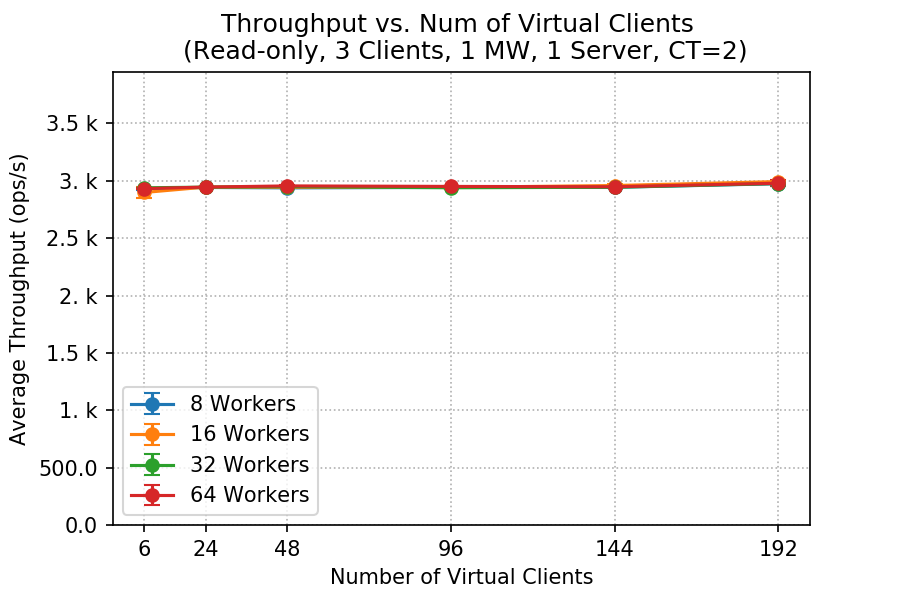
\includegraphics[width=1\linewidth]{figures/2_BaselineWithMW/one_mw/one_mw_tp_read_2018-12-06_23h08.png}
     \caption{Throughput of middleware}\label{one_mw_tp_read}
   \end{minipage}\hfill
   \begin{minipage}{0.48\textwidth}
     \centering
     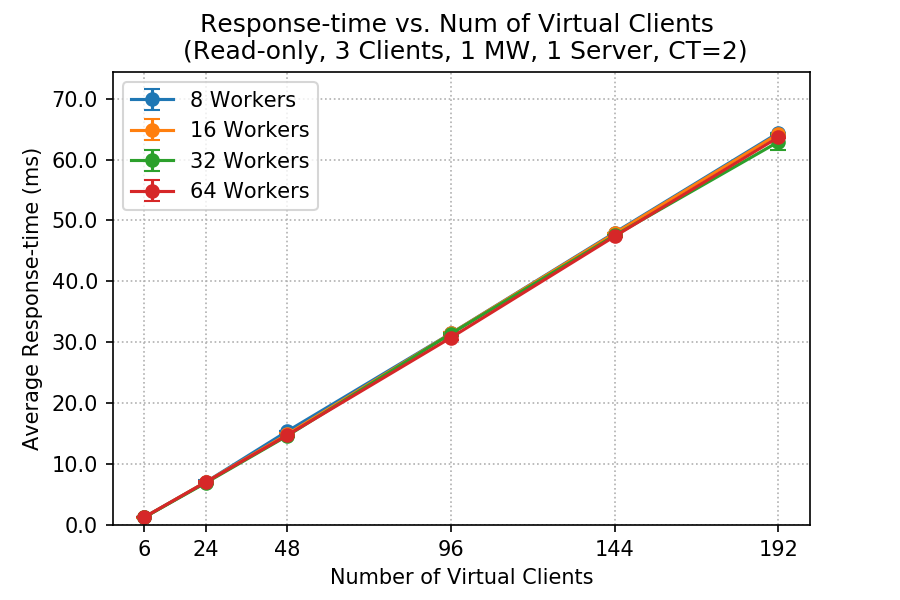
\includegraphics[width=1\linewidth]{figures/2_BaselineWithMW/one_mw/one_mw_rt_read_2018-12-06_23h08.png}
     \caption{Response time of middleware}\label{one_mw_rt_read}
   \end{minipage}
\end{figure}

%% explanation
% interactive law
The response time of the middleware is computed as the average time a request needs from the first encounter with the net-thread to the point where a worker thread sends the response back to the client. For the interactive law to hold, we can consider twice the network latency between the client and the middleware as the think time $Z$. 

% saturation & bottleneck
In Figure \ref{one_mw_tp_read} we can see that the saturation point for all worker settings is already reached at $6$ clients. The bottleneck of this setup is the outbound network bandwidth at the server, which can be seen in in Figure \ref{outbound_server_net_activity_one_mws}. Using \textit{iperf}, we checked that the maximum outbound network bandwidth of a server VM is 12.6 MBps, which is reached at $6$ clients and thus we don't see any under-saturation. The bottleneck also makes sense because of the large values the server has to send back for read-only workloads. Different number of workers reach the same maximum throughput, which supports the claim that bandwidth is the bottleneck because it is independent of the number of workers. 
\begin{figure}[H]
    \centering
	\includegraphics[scale=0.48]{figures/2_BaselineWithMW/one_mw/dstat_server_netsend_ratio_0:1_2018-12-06_23h08.png}
	\caption{Outbound network activity of the server VM.}
	\label{outbound_server_net_activity_one_mws}
\end{figure}
In the following, we want to support the claim by looking at the response time in more detail. Figure \ref{rt_breakdown_read_one_mw} shows that the response time stays the same for different number of workers, but the queue time shifts to the memcached RTT as we increase the number of workers. This is because we have a lower service rate of workers for small number of workers and thus requests wait longer in the middleware queue. If there are a lot of workers, requests are quickly dequeued, but they then congest at the server outbound queue and have to wait there instead because it is the bottleneck of the setup. 

\begin{figure}[H]
    \centering
	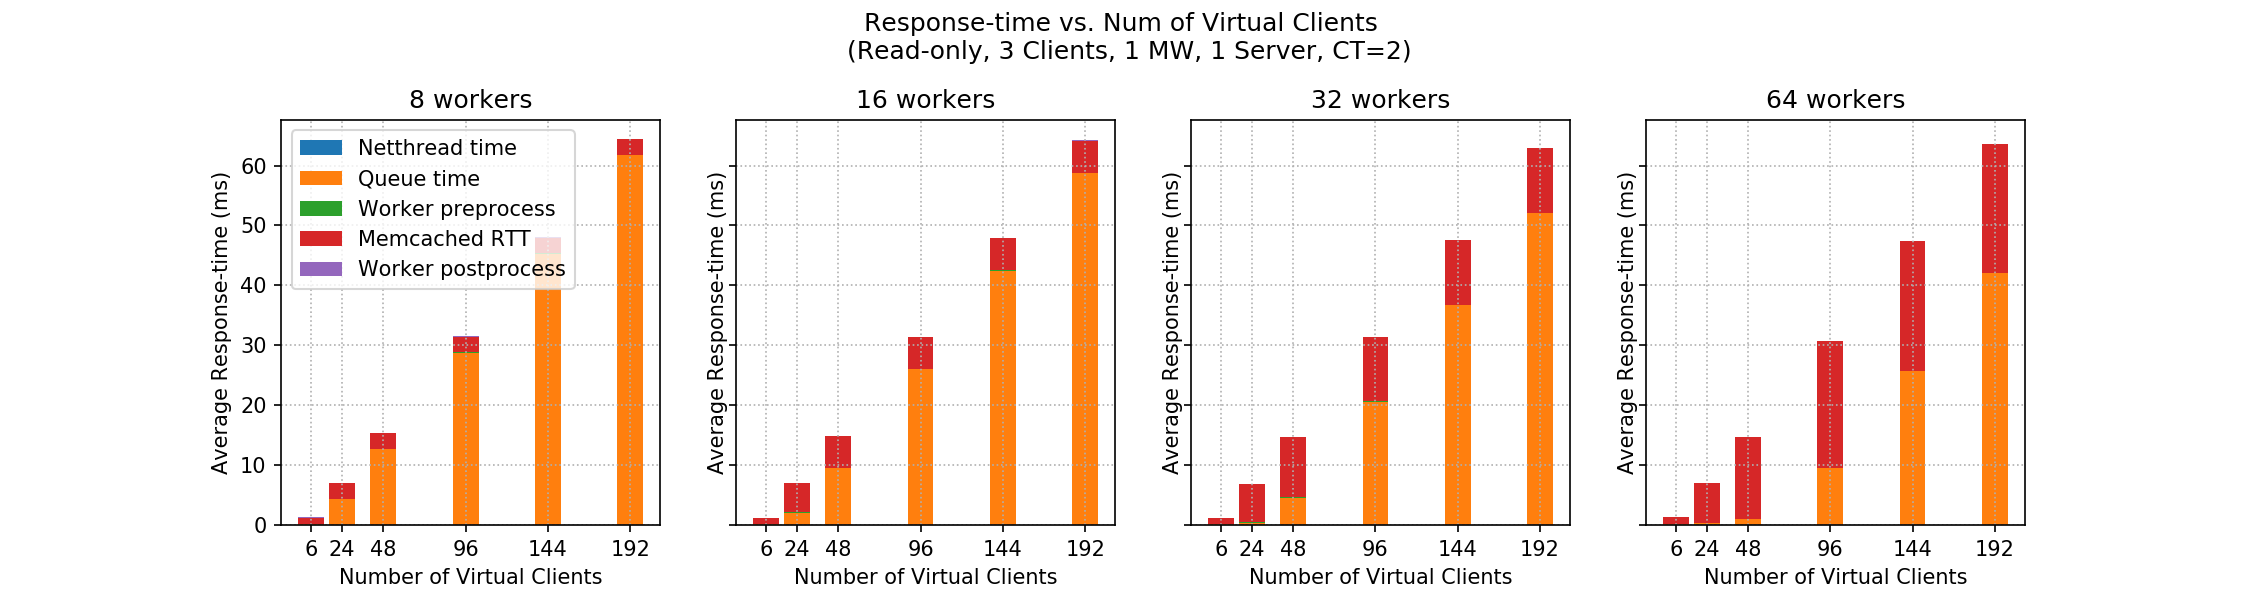
\includegraphics[scale=0.48,width=\linewidth]{figures/2_BaselineWithMW/one_mw/one_mw_rt_breakdown_read_2018-12-06_23h08.png}
	\caption{Response time breakdown of the read-only workloads.}
	\label{rt_breakdown_read_one_mw}
\end{figure}

$\bullet$ \textbf{Write-only load:} 
% plots
The throughput and response time measured on the middleware as a function of virtual clients for write-only workloads is shown in Figure \ref{one_mw_tp_write} and in Figure \ref{one_mw_rt_write}. 
\begin{figure}[ht]
   \begin{minipage}{0.48\textwidth}
     \centering
     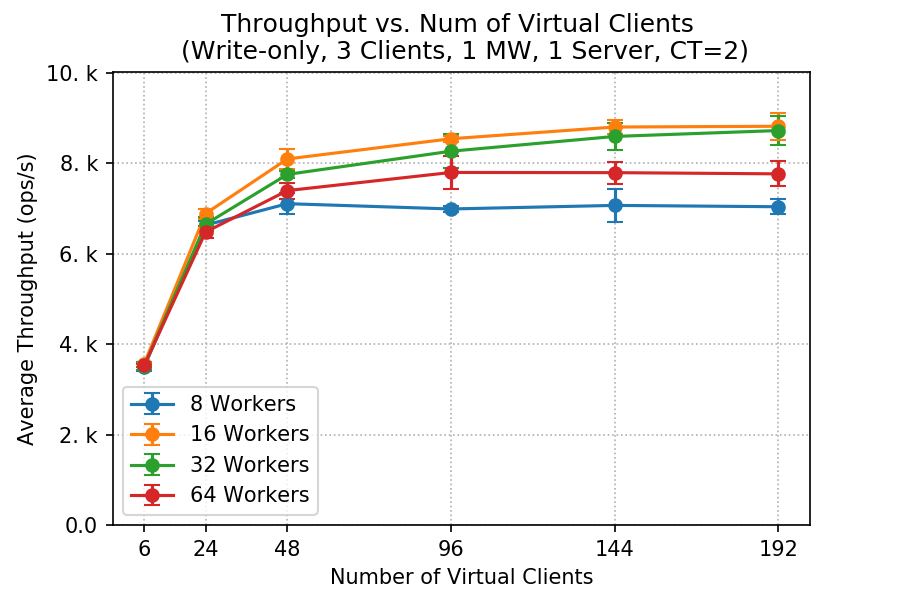
\includegraphics[width=1\linewidth]{figures/2_BaselineWithMW/one_mw/one_mw_mem_tp_write_2018-12-06_23h08.png}
     \caption{Throughput of middleware}\label{one_mw_tp_write}
   \end{minipage}\hfill
   \begin{minipage}{0.48\textwidth}
     \centering
     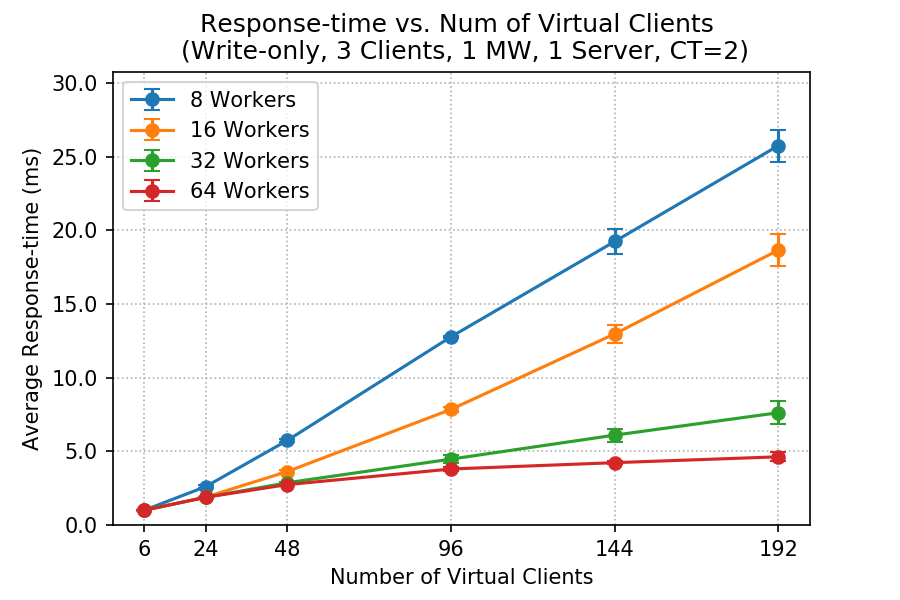
\includegraphics[width=1\linewidth]{figures/2_BaselineWithMW/one_mw/one_mw_rt_write_2018-12-06_23h08.png}
     \caption{Response time of middleware}\label{one_mw_rt_write}
   \end{minipage}
\end{figure}

%% explanation
% 8 and 16 worker threads
For \textbf{8 worker threads} saturation is reached at $24$ clients while for \textbf{16 worker threads} saturation is reached at $48$ clients as can be seen in Figure \ref{one_mw_tp_write} and \ref{one_mw_rt_write}. In both cases the bottleneck are the worker threads which cannot dequeue requests faster than they are enqueued by the net-thread. This can be verified by multiple metrics. First we can look at the average queue length for different number of clients. Figure \ref{queue_length_one_mw_write} shows that for 8 and 16 worker threads the queue length starts increasing more significantly at their saturation points. This happens because the arrival rate of requests into the queue is bigger than the overall service rate of the workers and thus requests start accumulating in the queue.   
\begin{figure}[H]
    \centering
	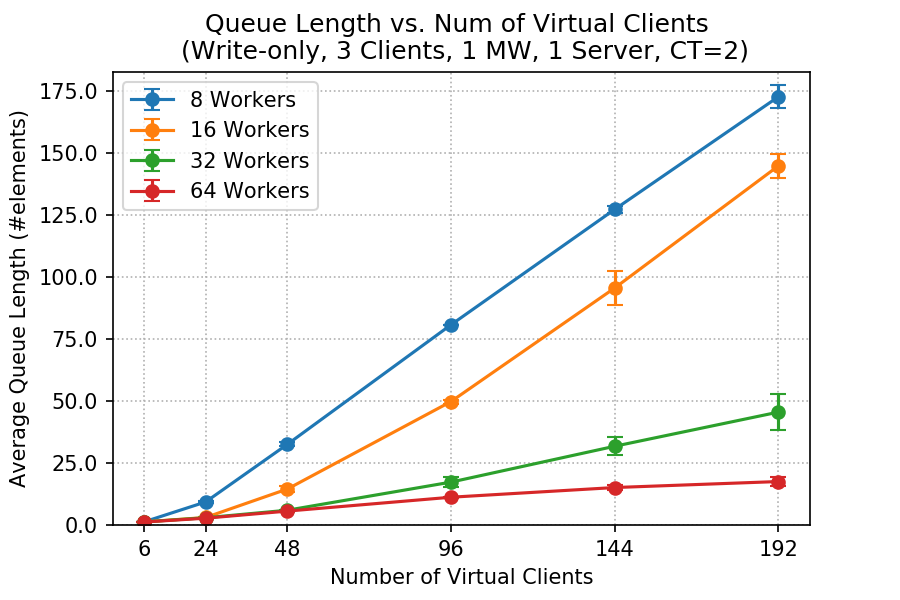
\includegraphics[scale=0.48]{figures/2_BaselineWithMW/one_mw/one_mw_queuelength_write_2018-12-06_23h08.png}
	\caption{Average queue length for write-only workloads.}
	\label{queue_length_one_mw_write}
\end{figure}
We can also look at the response time in the middleware in more detail. Figure \ref{rt_breakdown_write_one_mw} shows that for 8 and 16 worker threads, requests spend most of their time in the queue, and once dequeued they are processed quickly, which supports our claim. 
\begin{figure}[H]
    \centering
	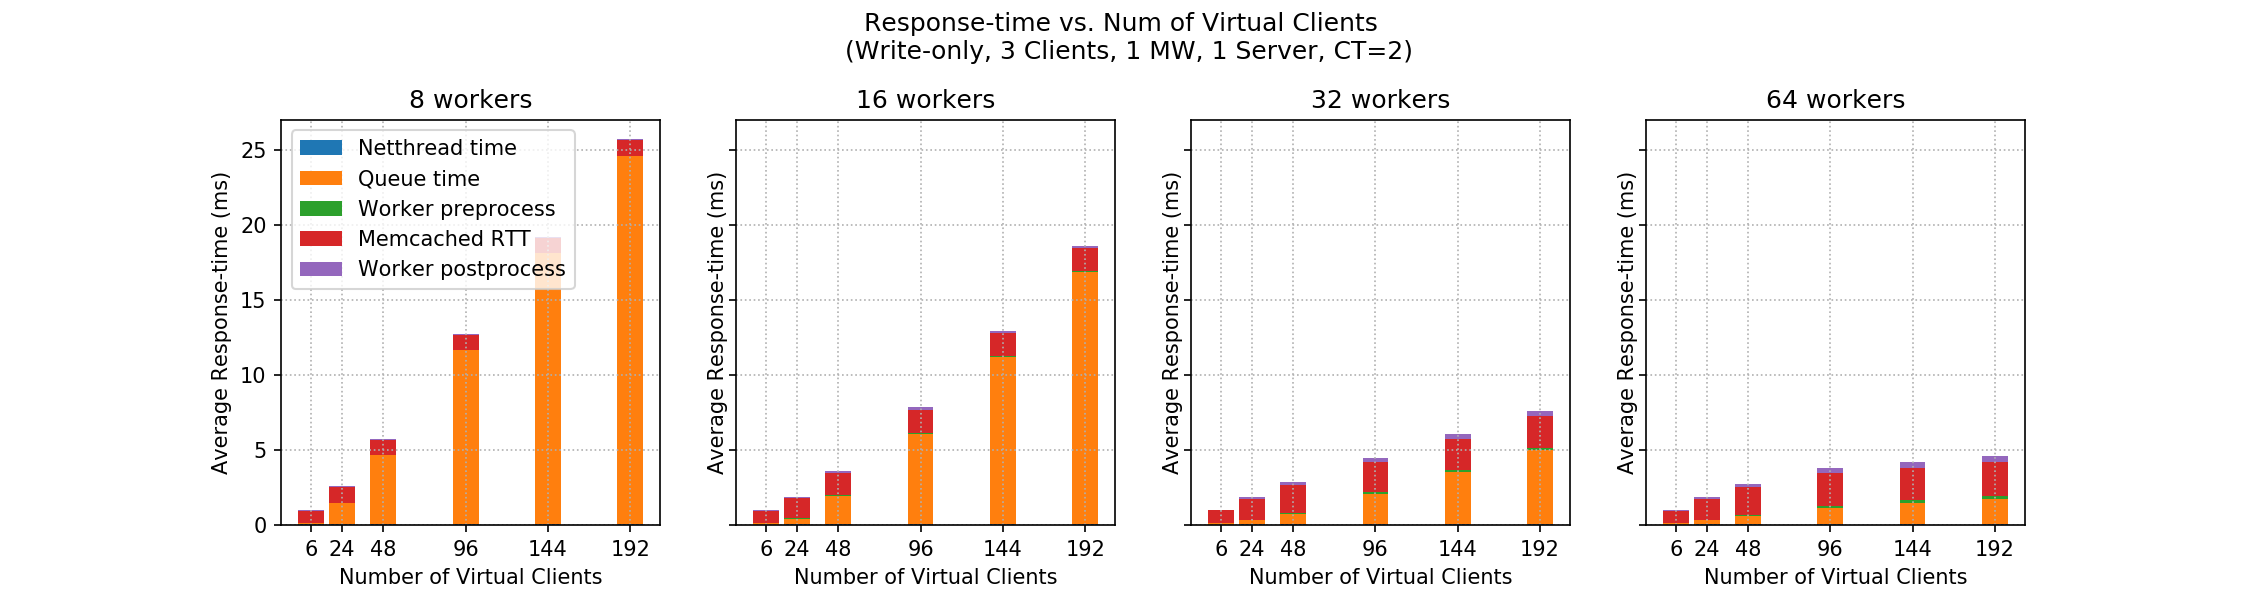
\includegraphics[scale=0.48,width=\linewidth]{figures/2_BaselineWithMW/one_mw/one_mw_rt_breakdown_write_2018-12-06_23h08.png}
	\caption{Response time breakdown of the write-only workloads.}
	\label{rt_breakdown_write_one_mw}
\end{figure}
% 32 and 64 worker threads
If we look at \textbf{32 and 64 worker threads}, first of all in Figure \ref{one_mw_tp_write} we see that in both cases saturation is reached at around 48 clients. The response time in the middleware for 32 and 64 worker threads is decreased in contrast to 8 and 16 worker threads as can be seen in Figure \ref{one_mw_rt_write}. This is because we increased the resources at the bottleneck, which are the worker threads. The queue time is decreased because the overall service rate of the workers is increased (Figure \ref{rt_breakdown_write_one_mw}).
Even though the response time at the middleware is decreased significantly, the overall response time measured at the clients (Figure \ref{rt_mem_write_one_mw}) did not, i.e. there is a new bottleneck now, which is the net-thread. Requests congest in the inbound network queue of the net-thread. 
This waiting time makes up roughly the difference between the response time measured on the middleware and on the client and is plotted separately in Figure \ref{netthread_queue_write}. We see that for 32 and 64 workers the time in front of the net-thread increases significantly at their saturation points.
\begin{figure}[H]
    \begin{minipage}{0.48\textwidth}
        \centering
	    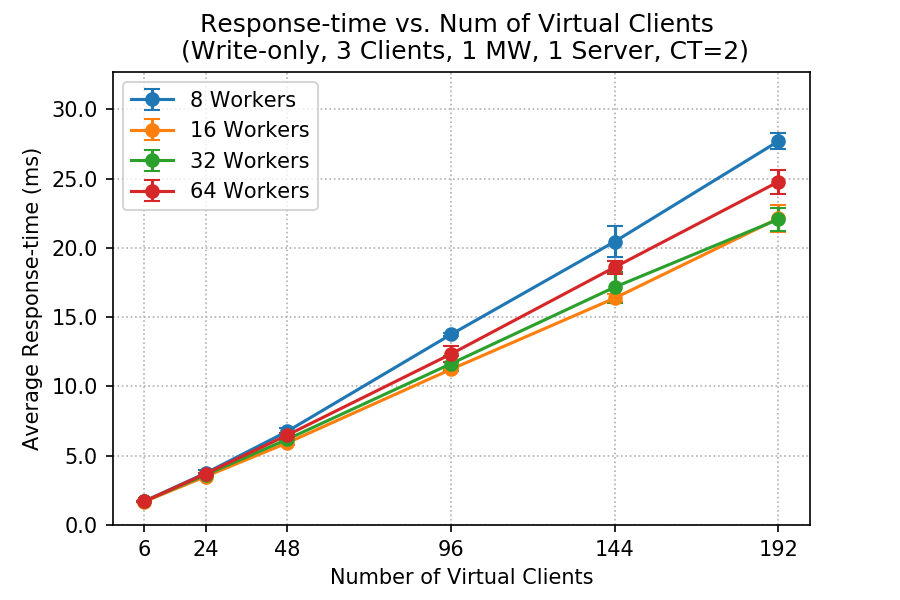
\includegraphics[scale=0.48]{figures/2_BaselineWithMW/one_mw/one_mw_mem_rt_write_2018-12-06_23h08.png}
	    \caption{Response time of the write-only workloads measured on client.}
	    \label{rt_mem_write_one_mw}
   \end{minipage}\hfill
   \begin{minipage}{0.48\textwidth}
        \centering
	    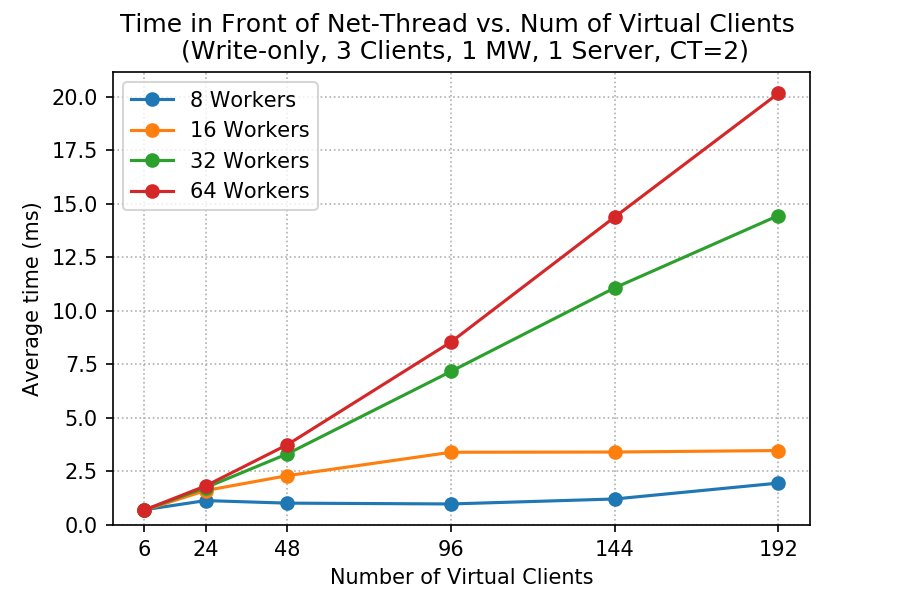
\includegraphics[scale=0.48]{figures/2_BaselineWithMW/one_mw/one_mw_rt_write_front_netthread_2018-12-06_23h08.png}
	    \caption{Average time spend in inbound network queue of net-thread.}
	    \label{netthread_queue_write}
   \end{minipage}
\end{figure}
The increase in inbound net-thread queue time for higher number of workers can be explained as follows: The more worker threads we have, the higher the overhead on the CPU i.e. more threads compete for the same resource and thus there are more context switches (verified with \textit{dstat}), which affects the performance of the net-thread because it gets less CPU time and can process fewer requests. Note that workers are allocated a priori in our system.

So even tough going from 16 to 32 worker threads removes the worker bottleneck and decreases queue time (Figure \ref{rt_breakdown_write_one_mw}), this time is compensated by the increased waiting time in front of the net-thread, and thus the throughput does not improve (Figure \ref{one_mw_tp_write}). Going from 32 to 64 worker threads has almost no effect on the response time at the middleware because already 32 worker threads were enough to handle the load. So we just have more net-thread waiting time because of the higher overhead on the CPU but without decreased queue time. This leads to a worse throughput than in the 32 worker thread case (Figure \ref{one_mw_tp_write}).


\subsection{Two Middlewares} \label{sec:baselineWithMWTwo}
% setup description
In this experiment we connect one load generator machine (two instances of memtier with CT=1) to two middlewares and use 1 memcached server. 
The overview of the experiment parameters is given in the following table:
\begin{center}
	\scriptsize{
		\begin{tabular}{|l|c|}
			\hline Number of servers                & 1                        \\ 
			\hline Number of client machines        & 3                        \\ 
			\hline Instances of memtier per machine & 2                        \\ 
			\hline Threads per memtier instance     & 1                        \\
			\hline Virtual clients per thread       & \{1,4,8,16,24,32,40\}       \\ 
			\hline Workload                         & Write-only and Read-only \\
			\hline Number of middlewares            & 2                        \\
			\hline Worker threads per middleware    & \{8,16,32,48\}              \\
			\hline Repetitions                      & 3                        \\ 
			\hline 
		\end{tabular}
	} 
\end{center}

$\bullet$ \textbf{Read-only load:} 
% plots
The throughput and response time as a function of virtual clients for read-only workloads is shown in Figure \ref{two_mws_tp_read} and in Figure \ref{two_mws_rt_read}. 
\begin{figure}[H]
   \begin{minipage}{0.48\textwidth}
     \centering
     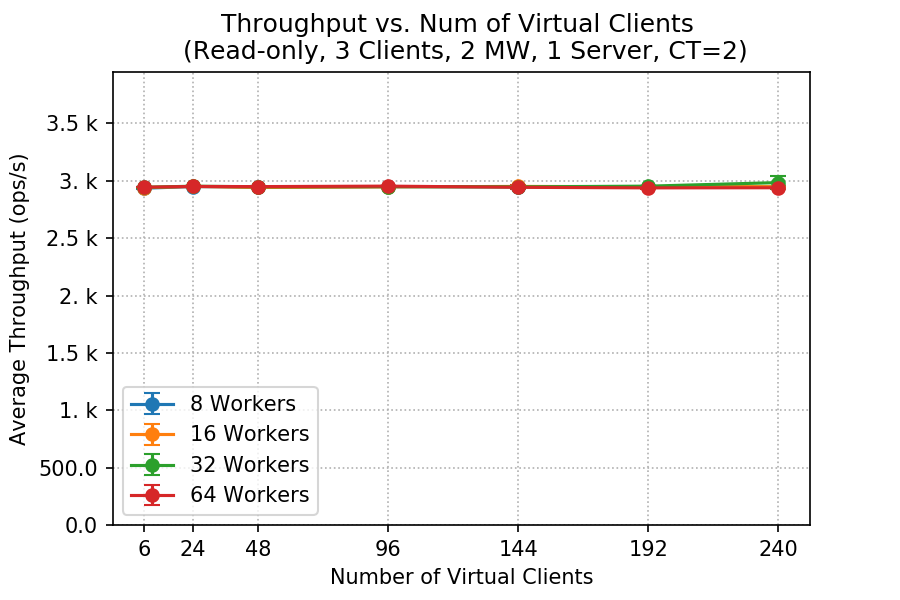
\includegraphics[width=1\linewidth]{figures/2_BaselineWithMW/two_mws/two_mws_tp_read_2018-12-07_09h02.png}
     \caption{Throughput of middlewares}\label{two_mws_tp_read}
   \end{minipage}\hfill
   \begin{minipage}{0.48\textwidth}
     \centering
     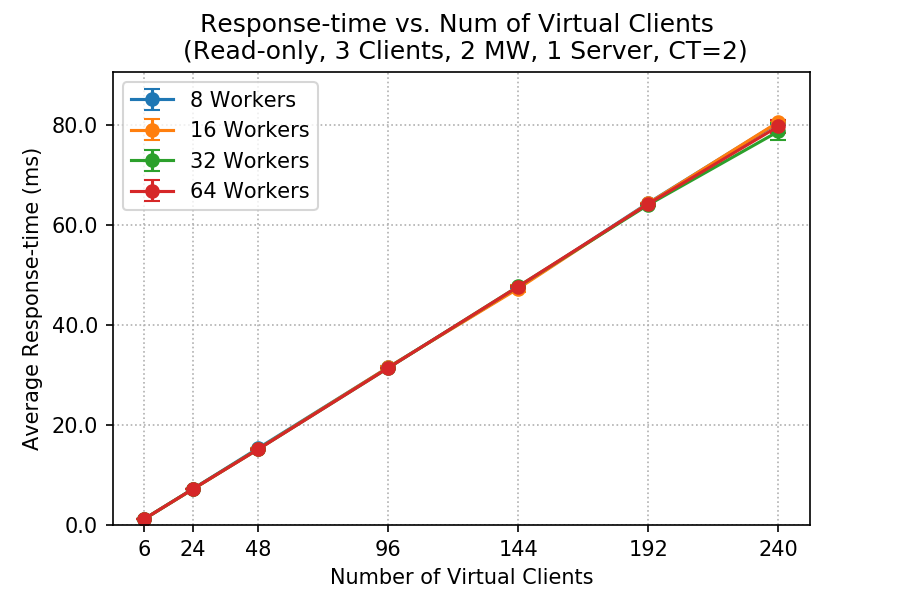
\includegraphics[width=1\linewidth]{figures/2_BaselineWithMW/two_mws/two_mws_rt_read_2018-12-07_09h02.png}
     \caption{Response time of middlewares}\label{two_mws_rt_read}
   \end{minipage}
\end{figure}

%% explanation
In Figure \ref{two_mws_tp_read} we can see that the saturation point for all worker settings is already reached at $6$ clients. The bottleneck of this setup is the same as for the one middleware case, namely the outbound network bandwidth at the server, which can be seen in in Figure \ref{outbound_server_net_activity_two_mws}. This also makes sense because going from one middleware to two middlewares does not improve the bottleneck at the server. The same reasoning done for the bottleneck analysis in the one middleware case applies here. 
\begin{figure}[H]
    \centering
	\includegraphics[scale=0.48]{figures/2_BaselineWithMW/two_mws/dstat_server_netsend_ratio_0:1_2018-12-07_09h02.png}
	\caption{Outbound network activity of the server VM.}
	\label{outbound_server_net_activity_two_mws}
\end{figure}
We can also look at the response time in more detail (Figure \ref{rt_breakdown_read_two_mws}) and see that increasing the number of workers shifts the time spent in the queue to the time spent in the outbound network queue of the server because of the server bandwidth bottleneck. 
\begin{figure}[H]
    \centering
	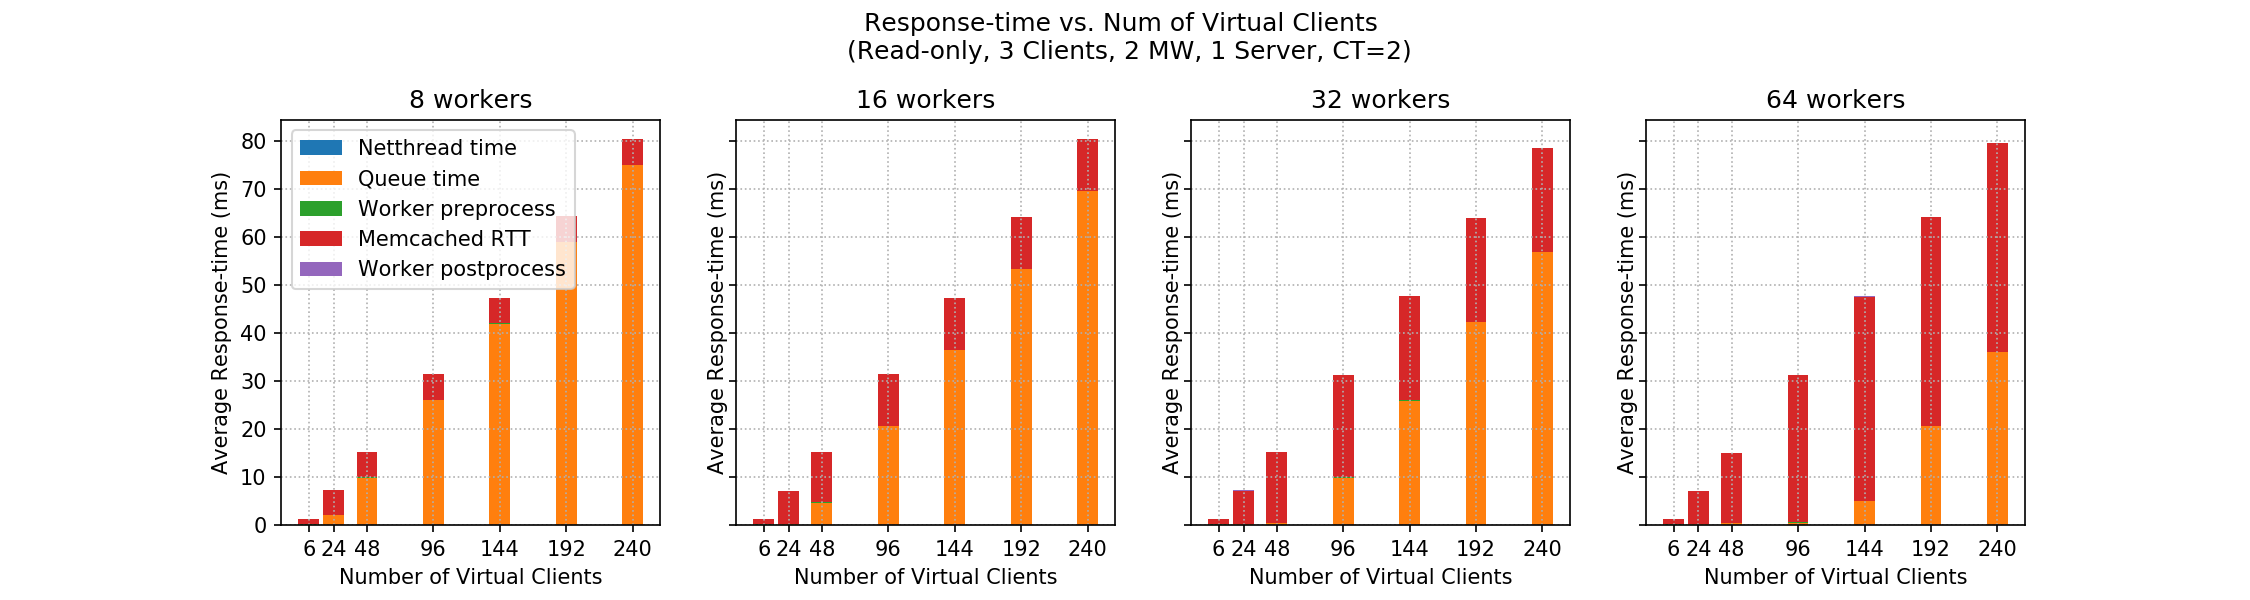
\includegraphics[scale=0.48,width=\linewidth]{figures/2_BaselineWithMW/two_mws/two_mws_rt_breakdown_read_2018-12-07_09h02.png}
	\caption{Response time breakdown of the read-only workloads.}
	\label{rt_breakdown_read_two_mws}
\end{figure}

$\bullet$ \textbf{Write-only load:} 
% plots
The throughput and response time as a function of virtual clients for write-only workloads is shown in Figure \ref{two_mws_tp_write} and in Figure \ref{two_mws_rt_write}. 
\begin{figure}[H]
   \begin{minipage}{0.48\textwidth}
     \centering
     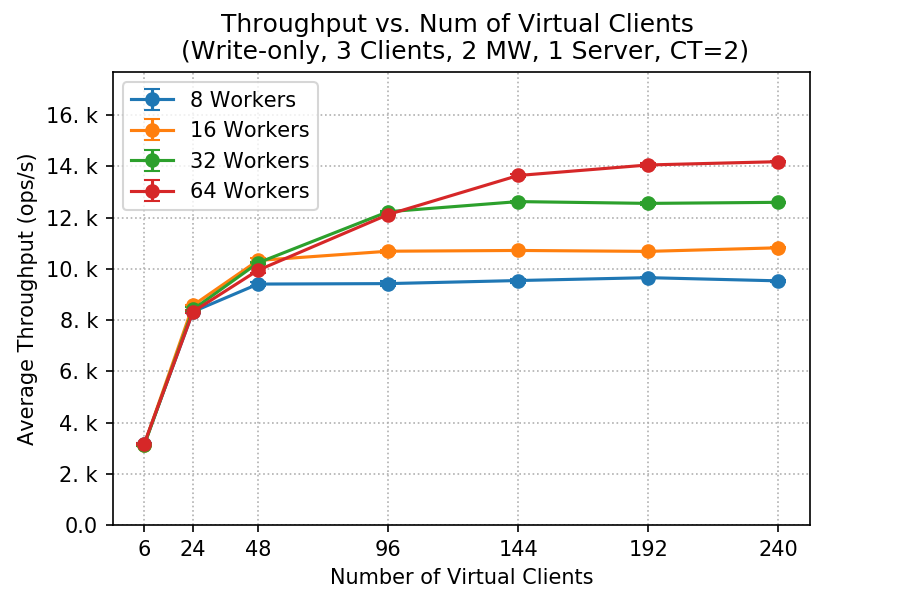
\includegraphics[width=1\linewidth]{figures/2_BaselineWithMW/two_mws/two_mws_tp_write_2018-12-07_09h02.png}
     \caption{Throughput of middlewares}\label{two_mws_tp_write}
   \end{minipage}\hfill
   \begin{minipage}{0.48\textwidth}
     \centering
     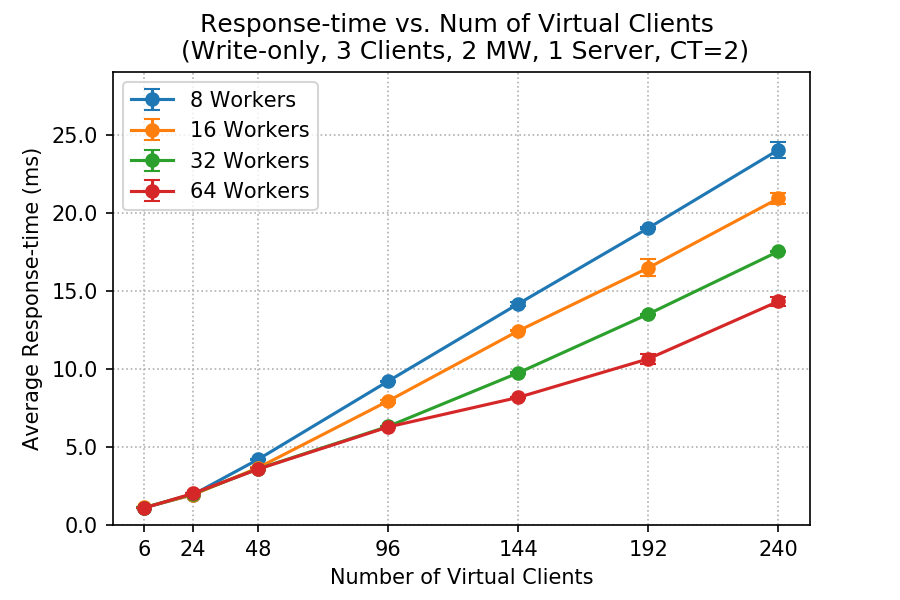
\includegraphics[width=1\linewidth]{figures/2_BaselineWithMW/two_mws/two_mws_rt_write_2018-12-07_09h02.png}
     \caption{Response time of middlewares}\label{two_mws_rt_write}
   \end{minipage}
\end{figure}
%% explanation
Looking at Figure \ref{two_mws_tp_write}, we see that saturation for 8 workers is reached at $24$ clients, for 16 workers at $48$ clients, for 32 clients at $96$ clients and for 64 workers at $144$ clients because at those points throughput starts to flatten. The saturation points are confirmed later in the analysis. In the one middleware case the net-thread is the bottleneck, but having two middlewares removes the net-thread bottleneck because we now have two net-threads sharing the same load. This can be confirmed by looking at the response time graph computed from the memtier outputs, which looks exactly the same as Figure \ref{two_mws_rt_write} plus 1-2 ms for the network latency between the client and the middleware. Thus no time is lost in front of the net-thread anymore. 
The bottleneck of this setup are the worker threads. To see this we can first look at the average queue length (Figure \ref{queue_length_two_mws_write}). The queue length starts increasing significantly at the mentioned saturation points.
We also checked the CPU utilization of the server VM (seen in Figure \ref{cpu_two_mws_write}) to verify that it does not reach full utilization which means that it is not the bottleneck of this setup.

%For 8, 16 and 32 workers the queue length starts increasing significantly at the mentioned saturation points. Actually for 64 worker threads the workers are not the bottleneck anymore but we claim that the single memcached thread is at its limit because it has to serve a lot of workers simultaneously.
%The server reaches almost full utilization at 144 clients as can be seen in Figure \ref{cpu_two_mws_write}.

\begin{figure}[H]
    \begin{minipage}{0.48\textwidth}
        \centering
	    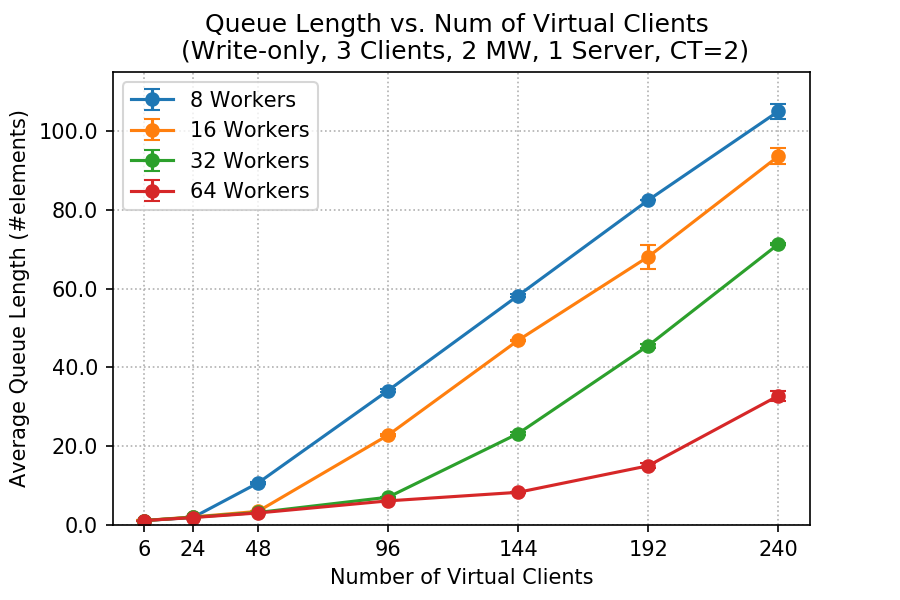
\includegraphics[scale=0.48]{figures/2_BaselineWithMW/two_mws/two_mws_queuelength_write_2018-12-07_09h02.png}
	    \caption{Average queue length for write-only workloads.}
	    \label{queue_length_two_mws_write}
    \end{minipage}\hfill
    \begin{minipage}{0.48\textwidth}
        \centering
	    \includegraphics[scale=0.48]{figures/2_BaselineWithMW/two_mws/dstat_server_cpu_ratio_1:0_2018-12-07_09h02.png}
	    \caption{CPU utilization of server VM for write-only workloads.}
	    \label{cpu_two_mws_write}
    \end{minipage}
\end{figure}

We can support our claim by additionally looking at the response time of the middleware in more detail (Figure \ref{rt_breakdown_write_two_mws}). We can see that the queue time starts increasing at the saturation points because the arrival rate of requests into the queue is higher then the service rate of the workers together. Note that if we fix the workers and look at the memcached RTT during saturation while increasing the clients, we see that it stays constant. That is because the workers are at full utilization and the arrival rate of requests into the memcached queue does not increase anymore, which further supports our claim that the workers are the bottleneck. 

%We can see that in deed for 8,16 and 32 workers the queue time makes up most of the response time. 64 workers have a higher service rate than arrival rate of requests into the queue and thus the queue time almost disappears. The bottleneck at the server leads to an increased memcached RTT for the 64 workers case which supports our claim. 
\begin{figure}[H]
    \centering
	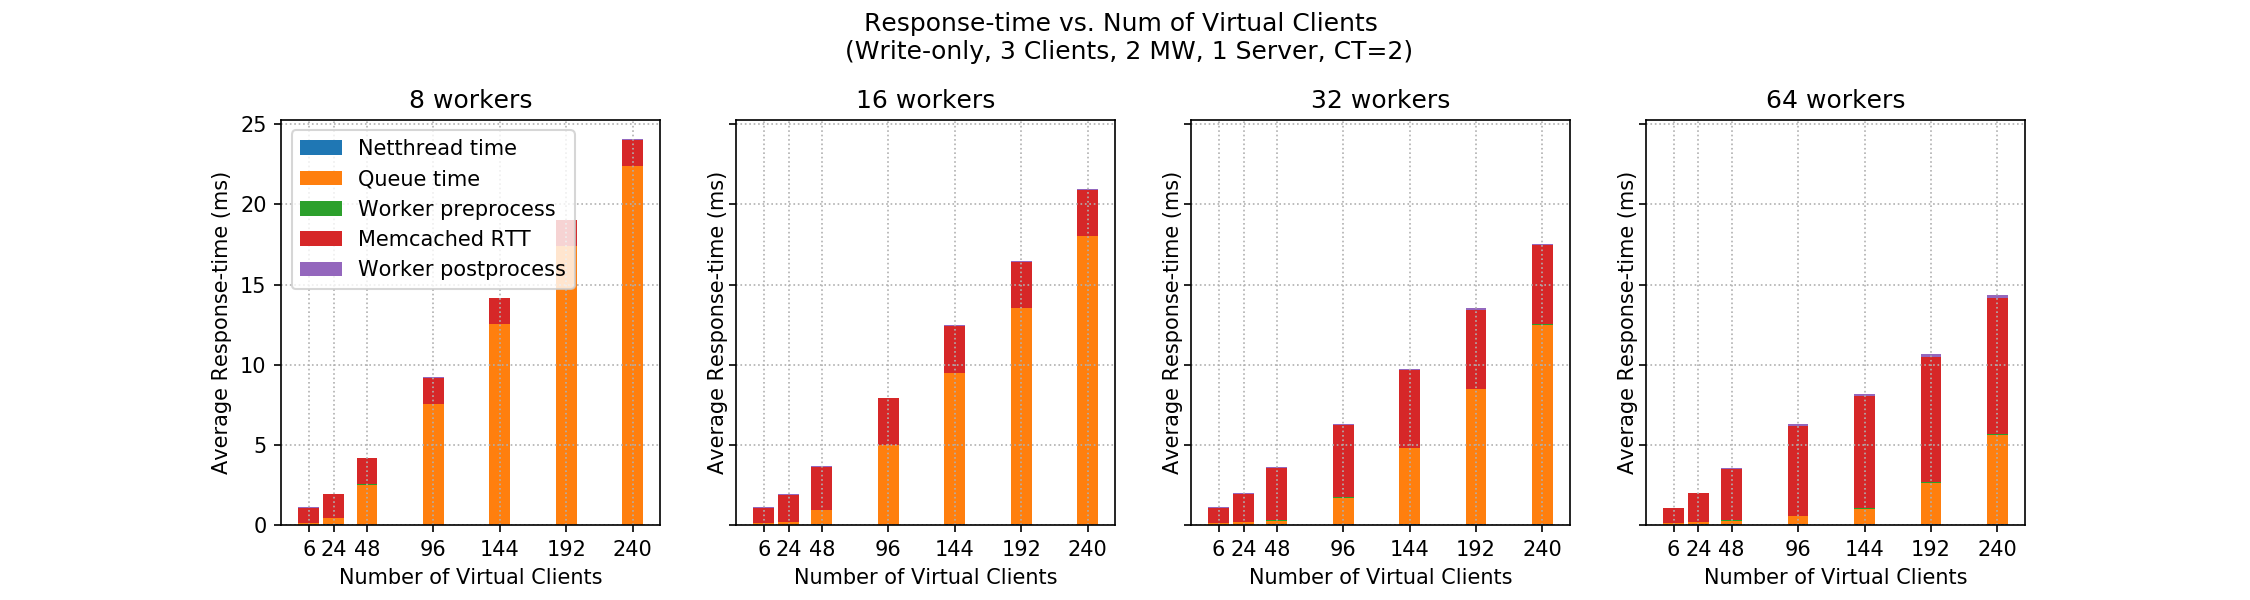
\includegraphics[scale=0.48,width=\linewidth]{figures/2_BaselineWithMW/two_mws/two_mws_rt_breakdown_write_2018-12-07_09h02.png}
	\caption{Response time breakdown of the write-only workloads.}
	\label{rt_breakdown_write_two_mws}
\end{figure}
\subsection{Summary}
\begin{center}
	{Maximum throughput for one middleware.}
	\begin{tabular}{|p{5.7cm}|p{2.1cm}|p{1.9cm}|p{1.9cm}|p{1.9cm}|}
		\hline                                & Throughput & Response time  & Average queue time & Miss rate  \\ 
		\hline Reads: Measured on middleware  &2'929 ops/s &1.26ms&      0.1ms &  0.0\%        \\ 
		\hline Reads: Measured on clients     & 2'925 ops/s&   2.06ms    & n/a   &   0.0\%    \\ 
		\hline Writes: Measured on middleware &   8'105 ops/s & 3.63ms         &    1.87ms      & n/a   \\ 
		\hline Writes: Measured on clients    &  8'097 ops/s&  5.93ms           & n/a                   & n/a      \\ 
		\hline 
	\end{tabular}
\end{center}

\begin{center}
	{Maximum throughput for two middlewares.}
	\begin{tabular}{|p{5.7cm}|p{2.1cm}|p{1.9cm}|p{1.9cm}|p{1.9cm}|}
		\hline                                & Throughput & Response time & Average queue time & Miss rate \\ 
		\hline Reads: Measured on middleware  &   2'935 ops/s &  1.18ms     &    0.08ms      & 0.0 \%   \\ 
		\hline Reads: Measured on clients     &   2'923 ops/s  &  2.06ms       & n/a         &   0.0 \%  \\ 
		\hline Writes: Measured on middleware &   13'645 ops/s &  8.18ms      &      0.97 ms              & n/a       \\ 
		\hline Writes: Measured on clients    &   13'603 ops/s   &10.6ms        & n/a                   & n/a     \\ 
		\hline 
	\end{tabular}
\end{center}
% table: 6 clients and 8 workers for read in both. 48 clients,16 workers for write one mw. 14 clients, 64 workers for write in two mw.
% conclusions
First note that again the maximum throughput is chosen by also taking the latency into consideration.
For the read-only workload, we choose the lowest number of clients (and workers) in both cases because the throughput remains the same while the response time increases with more clients. For the write-only workload and one middleware configuration, we choose $48$ clients and $16$ workers because going even further to $96$ clients would only increase the throughput by $5.5\%$ while increasing the response time more significantly by $89.5\%$. For the write-only workload and two middlewares configuration, we choose $144$ clients and $64$ workers because going to $192$ clients would only increase the throughput by $3\%$ but at the same time increase response time by $34.4\%$.

The response time difference between the client and the middleware is due to the time a request spends between a client and the middleware, which is not part of the response time measured at the middleware. 

If we look at the read-workloads, we see that increasing the number of middlewares does not improve the throughput. This is because the bottleneck is the outbound network bandwidth at the server, which puts a hard limit on the achievable throughput. 

If we look at the write-workloads, we see that going from one to two middlewares significantly increases the throughput. This is because the bottleneck in the one middleware case is the net-thread and having two net-threads allows them to share the same load, which reduces their utilization. 






\section{Throughput for Writes (90 pts)} \label{section:TpForWrites}
In this section we connect three load generating VMs to two middlewares and three memchached servers. We only run write-only workloads and we want to figure out the effects of replicating data to the servers. The experimental setup is the same as in the previous section.  

\subsection{Full System}
The overview of the experiment parameters is given in the following table:
\begin{center}
	\scriptsize{
		\begin{tabular}{|l|c|}
			\hline Number of servers                & 3          \\ 
			\hline Number of client machines        & 3          \\ 
			\hline Instances of memtier per machine & 2          \\ 
			\hline Threads per memtier instance     & 1          \\
			\hline Virtual clients per thread       & \{1,4,8,16,24,32,48\}    \\ 
			\hline Workload                         & Write-only \\
			\hline Number of middlewares            & 2          \\
			\hline Worker threads per middleware    & \{8,16,32,64\}   \\
			\hline Repetitions                      & 3   \\ 
			\hline 
		\end{tabular}
	} 
\end{center}
% plots
The throughput and response time as a function of virtual clients for write-only workloads is shown in Figure \ref{full_write_tp} and in Figure \ref{full_write_rt}. 
\begin{figure}[H]
   \begin{minipage}{0.48\textwidth}
     \centering
     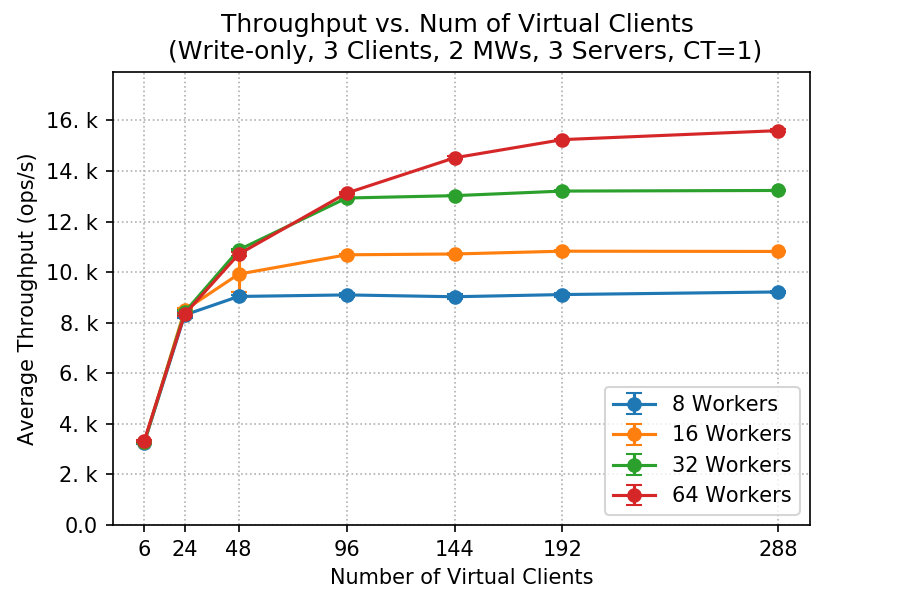
\includegraphics[width=1\linewidth]{figures/3_ThroughputForWrites/full_write_mw_tp_write_2018-11-09_13h02.png}
     \caption{Throughput of middlewares}\label{full_write_tp}
   \end{minipage}\hfill
   \begin{minipage}{0.48\textwidth}
     \centering
     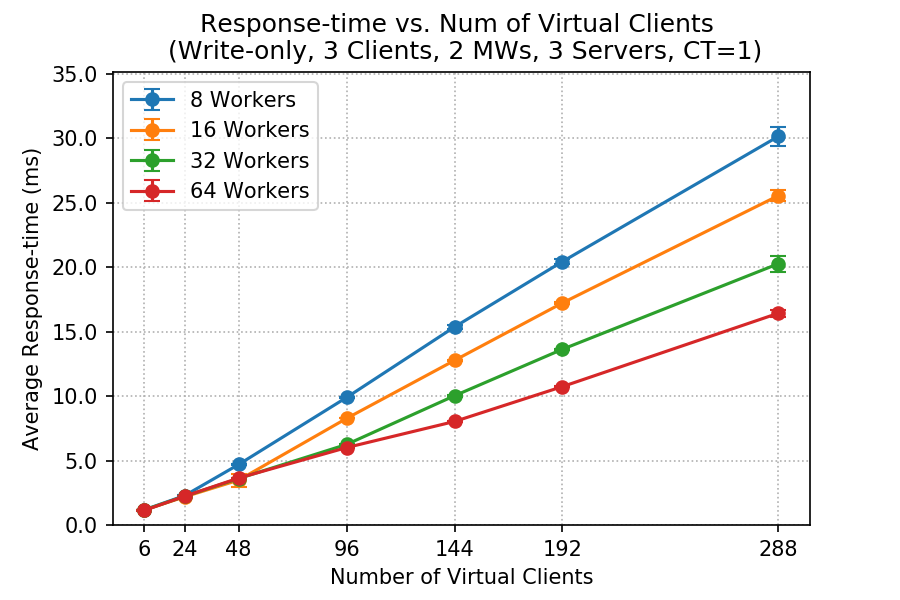
\includegraphics[width=1\linewidth]{figures/3_ThroughputForWrites/full_write_rt_write_2018-11-09_13h02.png}
     \caption{Response time of middlewares}\label{full_write_rt}
   \end{minipage}
\end{figure}

%% explanation
In Figure \ref{full_write_tp} and Figure \ref{full_write_rt} we can see that saturation for 8 workers is reached at 24 clients, for 16 workers at 48 clients, for 32 workers at 96 clients and for 64 workers at 192 clients because at those points throughput starts to flatten and we also see the response time increasing more significantly. 

First of all, we can compare the response time measured at the middleware with Section \ref{sec:baselineWithMWTwo} (write-only workload), where we have one instead of three servers. Comparing Figure \ref{two_mws_rt_write} and Figure \ref{full_write_rt} we see that the response time does slightly increase if we take three instead of one server, which makes sense because we have to additionally replicate the data in this experiment. A worker thread sends a Set request from the client to each server, one after the other, and then waits until all Set requests have been executed on all servers, which leads to a longer response time on the middleware. 

The bottleneck for all four worker configurations are the worker threads themselves. To see this we can first look at the average queue length (Figure \ref{queue_length_full_write}). We see that the queue length starts increasing significantly at the mentioned saturation points. We have queue congestion because the arrival rate into the queue is bigger than the combined service rate of the worker threads. 

\begin{figure}[H]
   \begin{minipage}{0.48\textwidth}
        \centering
	    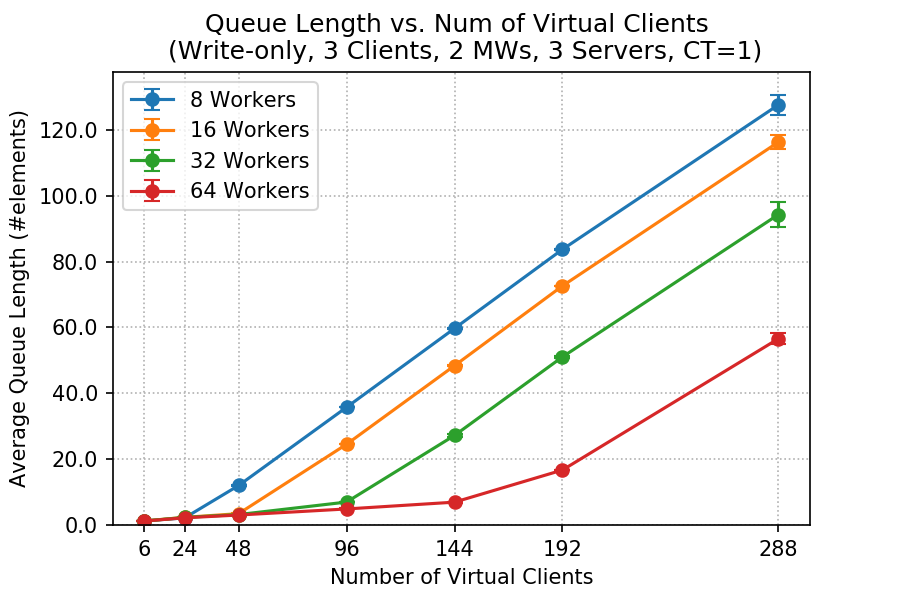
\includegraphics[scale=0.48]{figures/3_ThroughputForWrites/full_write_mw_queuelength_write_2018-11-09_13h02.png}
	    \caption{Average queue length.}
	    \label{queue_length_full_write}
   \end{minipage}\hfill
   \begin{minipage}{0.48\textwidth}
        \centering
	    \includegraphics[scale=0.48]{figures/3_ThroughputForWrites/dstat_mw_netsend_ratio_1:0_2018-11-09_13h02.png}
	    \caption{Outbound network activity of the middlewares.}
	    \label{outbound_mw_network_acitivity_full_write}
   \end{minipage}
\end{figure}
% look at outbound network bandwidth of middleware
We also checked the outbound network bandwidth at the middlewares because the middlewares have to send three times more data than in the one server case due to replication. Figure \ref{outbound_mw_network_acitivity_full_write} shows the outbound network activity of a middleware VM. We found out with \textit{iperf} that the maximum outbound bandwidth of a middleware VM is 100 MBps, which is almost reached for 64 workers. But since it is not reached at the saturation point, it is not the reason for saturation and thus not the bottleneck for the 64 workers case. 

We can support our bottleneck analysis by additionally looking at the response time of the middleware in more detail (Figure \ref{rt_breakdown_write_full_write}). We can also see that the queue time starts increasing at the saturation points.
The increase in waiting time for memcached (denoted as "Memcached RTT") for higher number of workers also makes sense because servers need to serve more workers simultaneously. 
\begin{figure}[H]
    \centering
	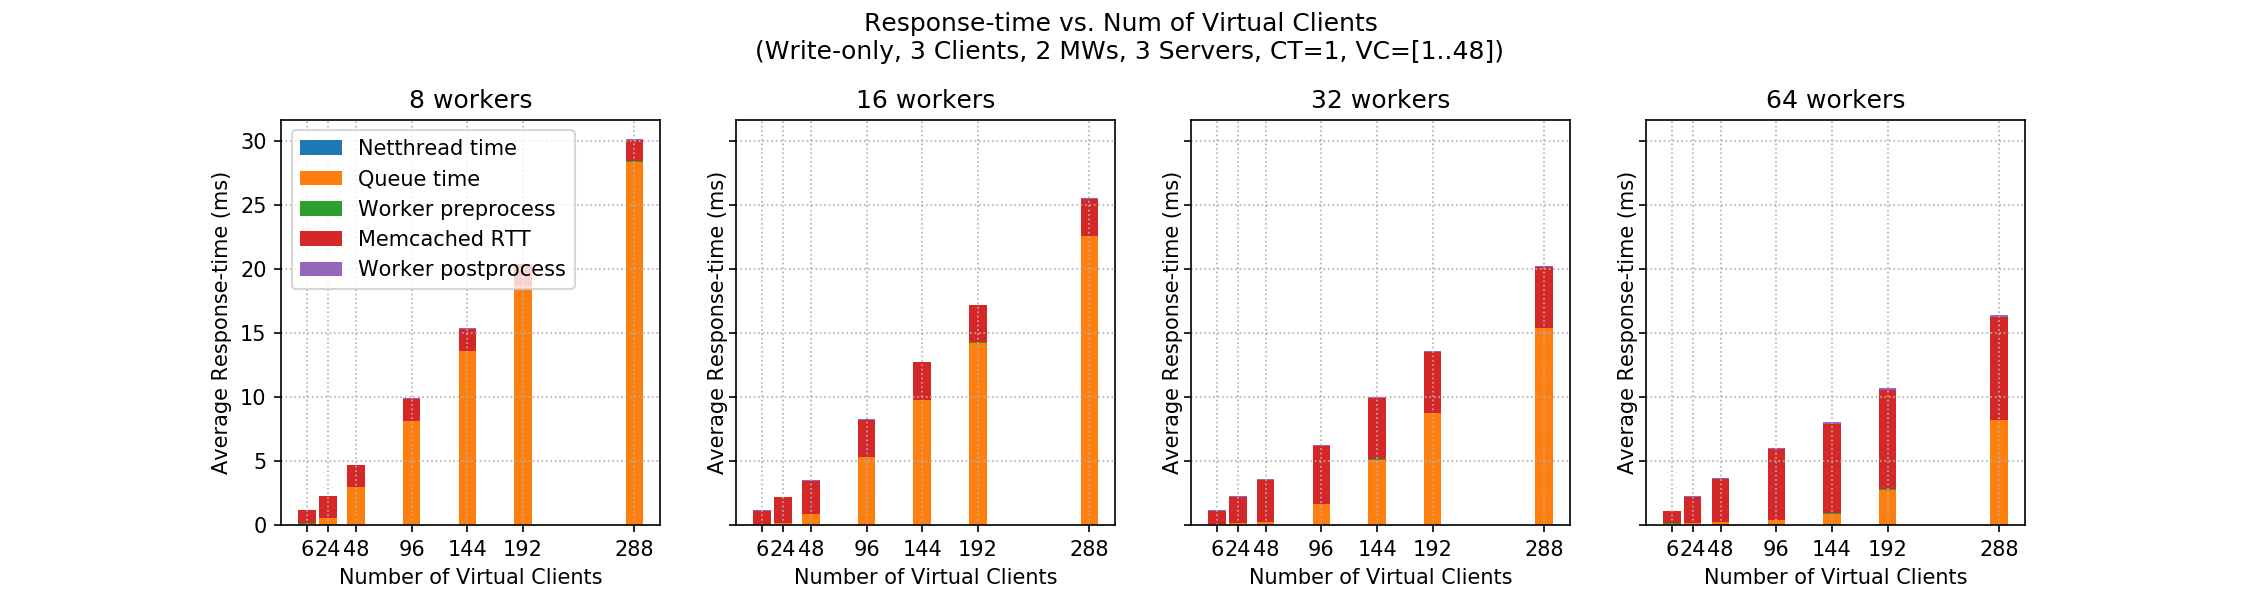
\includegraphics[scale=0.48,width=\linewidth]{figures/3_ThroughputForWrites/full_write_mw_rt_breakdown_write_2018-11-09_13h02.png}
	\caption{Response time breakdown.}
	\label{rt_breakdown_write_full_write}
\end{figure}

% analyze CPU utilization
%Our first guess is the CPU utilization of the servers because this is also the bottleneck for 64 worker threads in the one server case. Figure \ref{cpu_full_write} shows that this is not the case for three servers. We see that CPU utilization increases with more worker threads because the memcached threads have to maintain more connections in parallel and serve more requests but it is not the bottleneck.
%\begin{figure}[H]
%    \centering
%	\includegraphics[scale=0.48]{figures/3_ThroughputForWrites/dstat_server_cpu_ratio_1:0_2018-11-09_13h02.png}
%	\caption{CPU utilization of server VMs.}
%	\label{cpu_full_write}
%\end{figure}

% analyze mw bandwidth netsend
%Let us analyze the bottleneck for the \textbf{64 worker threads} setting. 
%Our guess is that the outbound network bandwidth at the middlewares is the bottleneck because the middlewares have to send %three times more data than in the one server case because of replication. Figure \ref{outbound_mw_network_acitivity_full_write} shows that this is indeed the case. We checked with \textit{iperf} that the maximum outbound bandwidth of a middleware VM is around 100 MBps which is reached in this case for the 64 worker setting.

\subsection{Summary}

\begin{center}
	{Maximum throughput for the full system}
	\begin{tabular}{|l|p{2.1cm}|p{2.1cm}|p{2.1cm}|p{2.1cm}|}
		\hline                                            & WT=8 & WT=16 & WT=32 & WT=64 \\ 
		\hline Throughput (Middleware)                    & 8'304 ops/s & 8'480 ops/s & 12'930 ops/s & 14'519 ops/s	       \\ 
		\hline Throughput (Derived from MW rt)            & 7'565 ops/s & 7'795 ops/s & 13'440 ops/s & 16'134 ops/s \\ 
		\hline Throughput (Client)                        &8'284 ops/s & 8'498 ops/s & 12'905 ops/s & 14'457 ops/s       \\ 
		\hline Average time in queue                      &0.54ms&0.14ms&1.59ms&0.8ms	 \\ 
		\hline Average length of queue                    &2.16 & 2.32 & 6.97 & 6.93 \\ 
		\hline Average time waiting for memcached         & 1.67ms  & 1.98ms & 4.51ms & 6.99ms	 \\ 
		\hline 
	\end{tabular}
\end{center}
% choice of configurations that give max throughput
The configurations that give maximal throughput are chosen such that a good trade-off between the throughput and latency is achieved. For 8 workers, 24 clients were chosen because going from 24 to 48 clients would increase response time by $84\%$, while only increasing throughput by $8.8\%$. For 16 workers, also 24 clients were chosen because going from 24 clients to 48 clients would increase response time by $55\%$, while only increasing throughput by $16\%$. For 32 workers, 96 clients were chosen because going from 96 to 144 clients would increase response time by $50\%$, while only increasing throughput by less than $1\%$. For 64 workers, 144 clients were chosen because going from 144 to 288 clients would increase response time by $28\%$, while only increasing throughput by $5\%$.

% interactive law
The throughput can be derived from the MW response time in two ways using the interactive law: Either we consider the round-trip time between the MWs and the clients as the waiting time Z or we adjust the number of requests N by subtracting the average number of requests that are between the clients and the middlewares. We choose the first approach and average the ping times between the clients and the middlewares to get an average round-trip time of 0.8915ms. 
% explain
For 64 workers the throughput derived from the middleware response time is significantly overestimated. This is because the difference between the response time measured at the client and at the middleware is larger than the network latency between them and thus the think time Z is chosen too small. This difference includes the time a request waits in front of the net-thread. The more worker threads there are, the more threads compete for the same resource, which slows down the net-thread.

% Draw conclusions on the state of your system for a variable number of worker threads.
The highest throughput is reached with 64 worker threads. This is because the workers are the bottleneck in this setup and in general increasing the resource at a bottleneck increases the throughput of a system. Thus we achieve highest throughput with the highest number of workers.
With 64 worker threads and high enough load, the maximum outbound network bandwidth of the middleware VMs is almost reached (Figure \ref{outbound_mw_network_acitivity_full_write}) which means that going beyond 64 workers would not significantly increase the throughput anymore in this setup. In order to reduce the network send activity of the middleware VMs such that one can increase the throughput even more, one would have to either increase the number of middlewares or decrease the replication factor of the key-value pairs.



\section{Gets and Multi-gets (90 pts)}
In this section we connect three load generating VMs to two middlewares and three memchached servers. We want to understand the effects of increasing the multi-get size on the performance of system. In addition, we analyze if sharding the multigets improves the performance.

\subsection{Sharded Case}
The overview of the experiment parameters is given in the following table:
\begin{center}
	\scriptsize{
		\begin{tabular}{|l|c|}
			\hline Number of servers                & 3                       \\ 
			\hline Number of client machines        & 3                       \\ 
			\hline Instances of memtier per machine & 2                       \\ 
			\hline Threads per memtier instance     & 1                       \\
			\hline Virtual clients per thread       & 2     		            \\ 
			\hline Workload                         & ratio=1:$<$Multi-Get size$>$             \\
			\hline Multi-Get behavior               & Sharded                 \\
			\hline Multi-Get size                   & \{1,3,6,9\}                 \\
			\hline Number of middlewares            & 2                       \\
			\hline Worker threads per middleware    & 64 \\
			\hline Repetitions                      & 3                \\ 
			\hline 
		\end{tabular}
	} 
\end{center}

% plots
If sharding is activated, the keys inside the multiget requests are evenly split by the workers and distributed among the servers.
The average response time measured on the client as a function of the multiget size and the percentiles for the sharded case are shown in Figures \ref{sharded_rt} and \ref{sharded_percentiles}.
% data: [2018-11-22_18h12]
\begin{figure}[H]
   \begin{minipage}{0.48\textwidth}
     \centering
     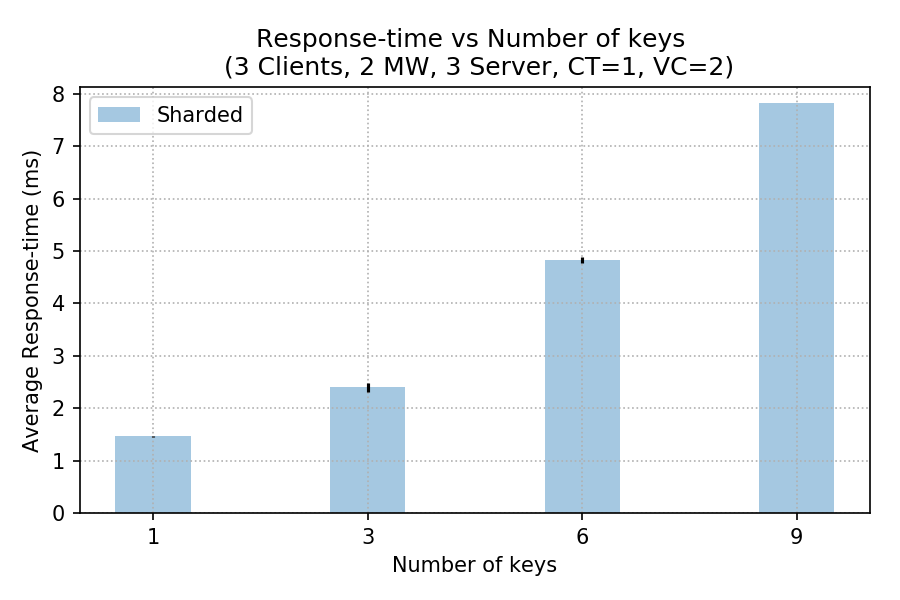
\includegraphics[width=1\linewidth]{figures/4_GetsAndMultigets/mem_rt_sharded_2018-11-22_18h12.png}
     \caption{Response time measured on clients.}\label{sharded_rt}
   \end{minipage}\hfill
   \begin{minipage}{0.48\textwidth}
     \centering
     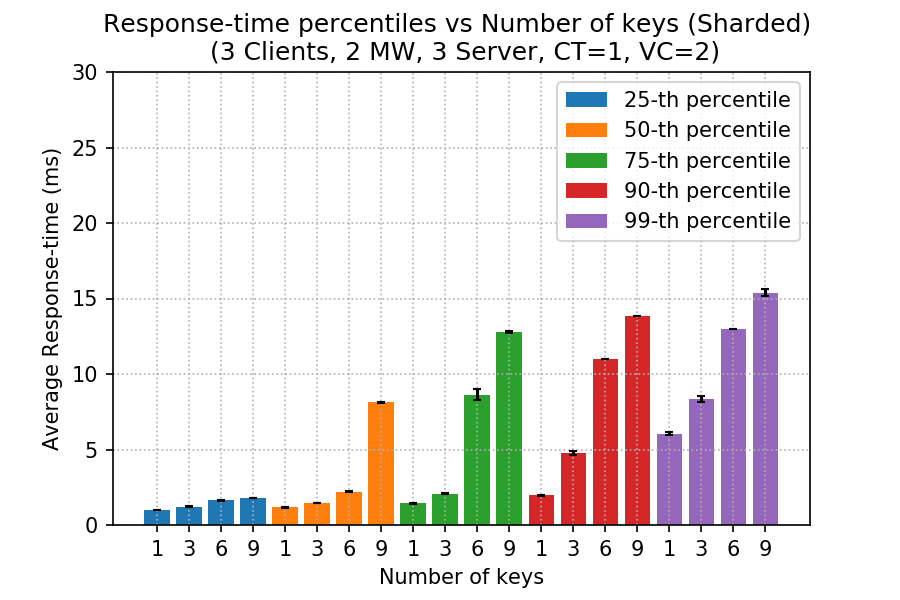
\includegraphics[width=1\linewidth]{figures/4_GetsAndMultigets/mem_perc_sharded_2018-11-22_18h12.png}
     \caption{Response time percentiles measured on client.}\label{sharded_percentiles}
   \end{minipage}
\end{figure}
First of all note that since we are in a closed system and we only have 12 clients, at least 52 workers will be idle at any moment in time. This is not optimal because threads use up memory and we establish more connections to servers than necessary (this depends on how the middleware has been implemented, but in our case the threads are started a priori). 

% bottleneck analysis
For 3, 6 and 9 keys the bottleneck is the outbound network bandwidth at the server VMs, as can be seen in Figure \ref{sharded_netsend_server}. Note that the maximal outbound network bandwidth of a server VM is 12 MBps.
For 1 key, the system is under-saturated because no component reaches full utilization. We checked the CPU usage of the VMs, the network send activity of the VMs, the response time breakdown in the middleware, the average queue length and we also have enough workers because at least 52 workers are always idle.\footnote{Those plots are not included in the report to keep it concise, but they can be found in the repository.} Thus for the 1 key case, the number of clients could be further increased to reach better performance regarding throughput.

\begin{figure}[H]
   \begin{minipage}{0.48\textwidth}
    \centering
	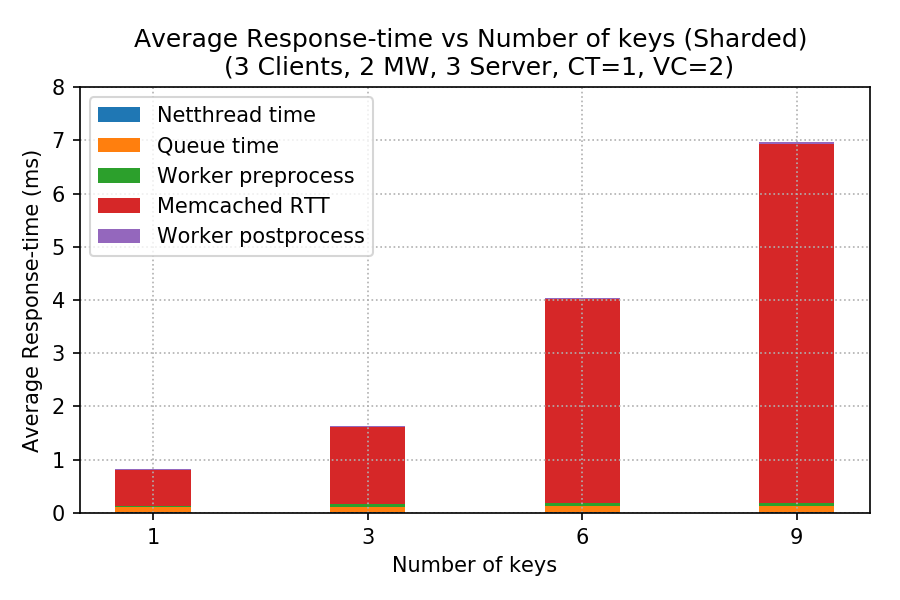
\includegraphics[scale=0.48]{figures/4_GetsAndMultigets/rt_breakdown_sharded_2018-11-22_18h12.png}
	\caption{Response time breakdown at middleware.}
	\label{rt_breakdown_sharded}
   \end{minipage}\hfill
   \begin{minipage}{0.48\textwidth}
     \centering
     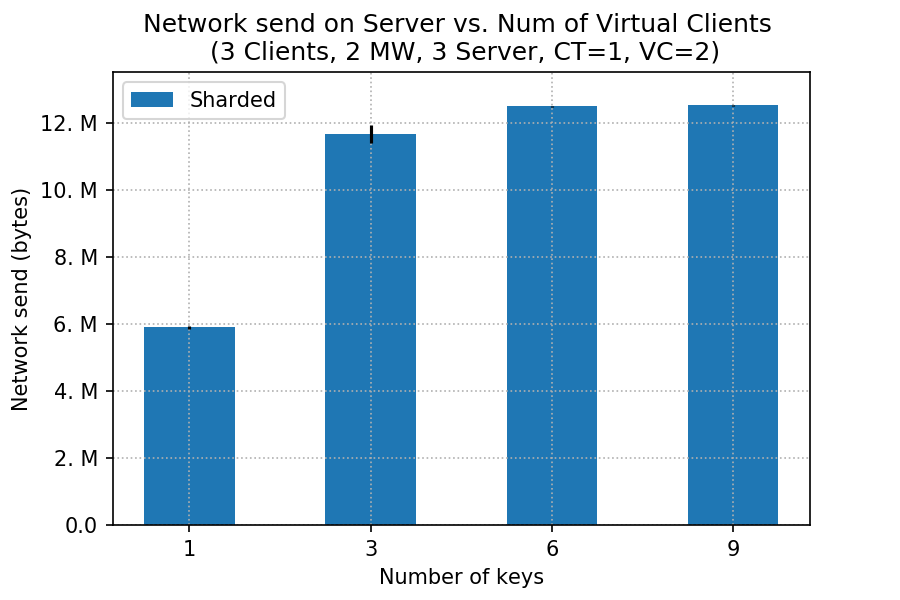
\includegraphics[width=1\linewidth]{figures/4_GetsAndMultigets/dstat_server_netsend_sharded_True_2018-11-22_18h12.png}
     \caption{Network send activity on a server VM.}\label{sharded_netsend_server}
   \end{minipage}
\end{figure}
If we look at the response time breakdown at the middleware in Figure \ref{rt_breakdown_sharded}, we can see that the memcached RTT makes up most of the time. The memcached RTT mainly consists of the network latency between the middleware and the server, the waiting time at the server because of the bandwidth bottleneck and the time it takes the server to write the response into the network. We see that the average response time on the middleware (Figure \ref{rt_breakdown_sharded}) is lower than on the client (Figure \ref{sharded_rt}), which is because of the network latency between the client and middleware. We also see that in Figures \ref{sharded_rt} and \ref{rt_breakdown_sharded}, the response time increases with the number of keys. This is because the server has to write more data into the network and also has to process more data. Note that the memcached RTT is what significantly increases the overall response time with increasing key size. 

If we look at the percentile plot (Figure \ref{sharded_percentiles}), we see that individual percentiles increase with increasing number of keys for the same reason as the average response time increases with the number of keys. 
The percentile plot will be further explained in comparison with the plot of the non-sharded case and in subsection \ref{sub:hist}.

\subsection{Non-sharded Case}
The overview of the experiment parameters is given in the following table:
\begin{center}
	\scriptsize{
		\begin{tabular}{|l|c|}
			\hline Number of servers                & 3                       \\ 
			\hline Number of client machines        & 3                       \\ 
			\hline Instances of memtier per machine & 2                       \\ 
			\hline Threads per memtier instance     & 1                       \\
			\hline Virtual clients per thread       & 2     		            \\ 
			\hline Workload                         & ratio=1:$<$Multi-Get size$>$             \\
			\hline Multi-Get behavior               & Non-Sharded                 \\
			\hline Multi-Get size                   & \{1,3,6,9\}                 \\
			\hline Number of middlewares            & 2                       \\
			\hline Worker threads per middleware    & 64 \\
			\hline Repetitions                      & 3                \\ 
			\hline 
		\end{tabular}
	} 
\end{center}

% plots
The average response time measured on the client as a function of the multiget size and the percentiles for the non-sharded case is shown in Figure \ref{nonsharded_rt} and \ref{nonsharded_percentiles}.
% data: [2018-11-22_18h12]
\begin{figure}[H]
   \begin{minipage}{0.48\textwidth}
     \centering
     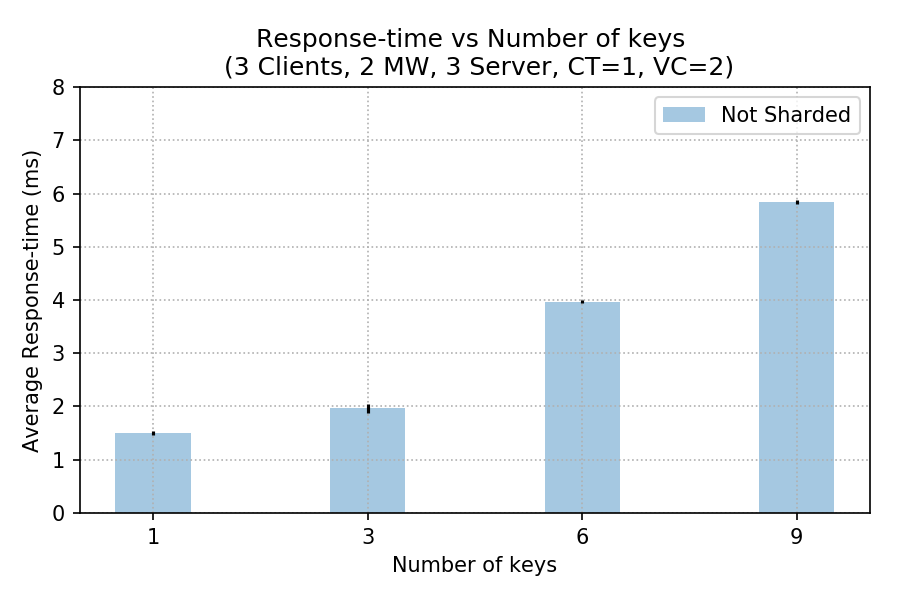
\includegraphics[width=1\linewidth]{figures/4_GetsAndMultigets/mem_rt_nonsharded_2018-11-22_18h12.png}
     \caption{Response time measured on clients.}\label{nonsharded_rt}
   \end{minipage}\hfill
   \begin{minipage}{0.48\textwidth}
     \centering
     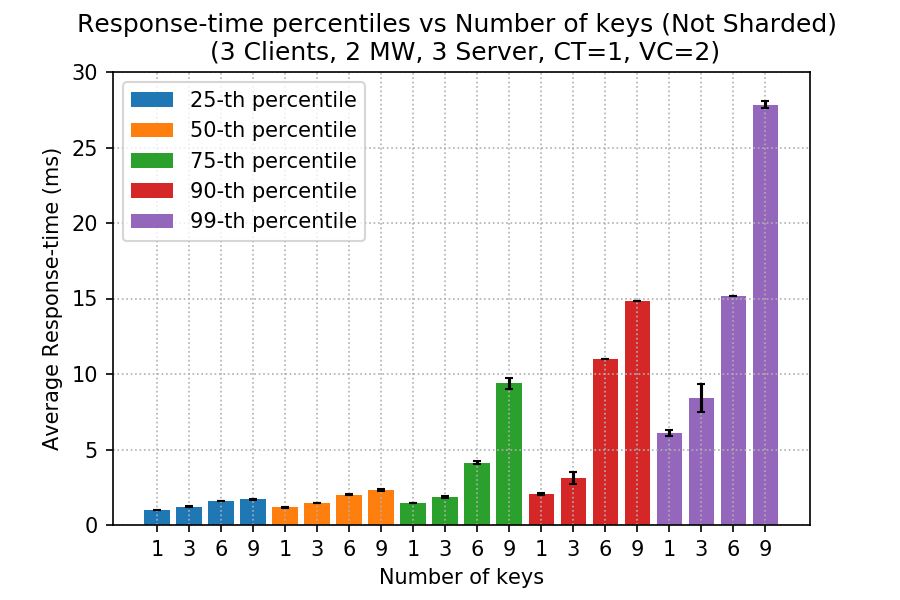
\includegraphics[width=1\linewidth]{figures/4_GetsAndMultigets/mem_perc_nonsharded_2018-11-22_18h12.png}
     \caption{Response time percentiles measured on client.}\label{nonsharded_percentiles}
   \end{minipage}
\end{figure}
For the non-sharded case we have the same bottleneck as in the sharded case, namely the outbound network bandwidth of the server VMs (see Figure \ref{nonsharded_netsend_server}). The same reasoning done in the sharded subsection applies here. For 1 key, the system is also under-saturated because no component reaches full utilization.  The memcached RTT makes up most of the response time measured at the middleware (Figure \ref{rt_breakdown_nonsharded}) and the response times increase with the key size for the same reasons. In this subsection I mainly focus on comparing the plots with their sharded counterpart. 


\begin{figure}[ht]
   \begin{minipage}{0.48\textwidth}
    \centering
	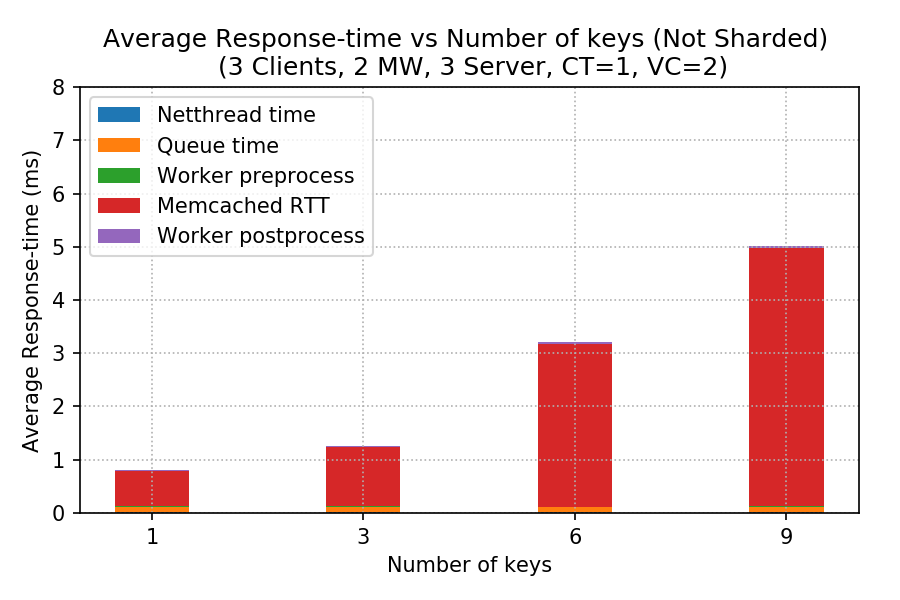
\includegraphics[scale=0.48]{figures/4_GetsAndMultigets/rt_breakdown_notsharded_2018-11-22_18h12.png}
	\caption{Response time breakdown at middleware.}
	\label{rt_breakdown_nonsharded}
   \end{minipage}\hfill
   \begin{minipage}{0.48\textwidth}
     \centering
     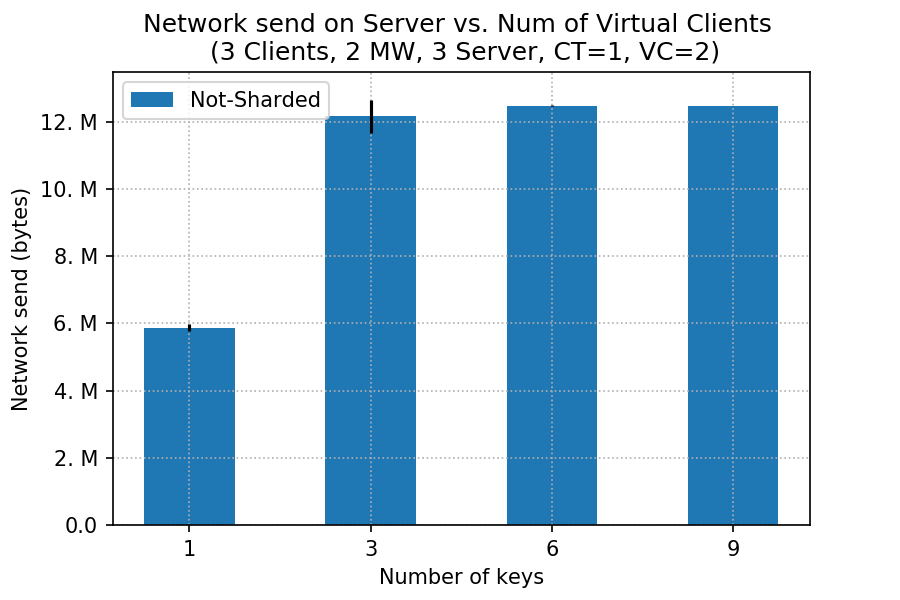
\includegraphics[width=1\linewidth]{figures/4_GetsAndMultigets/dstat_server_netsend_sharded_False_2018-11-22_18h12.png}
     \caption{Network send activity on a server VM.}\label{nonsharded_netsend_server}
   \end{minipage}
\end{figure}
First of all, looking at the requests with one key (Figures \ref{sharded_rt} and \ref{nonsharded_rt}), we see very similar response times for the sharded and non-sharded case because for one key the sharding behaves the same as for non-sharding.  For 3, 6 and 9 keys, we can observe that the average response times are higher in the sharded case than in the non-sharded case (Figures \ref{sharded_rt} and \ref{nonsharded_rt}). This is because in the sharded case a worker has to wait for a response from all servers, i.e. the response time is bound by the slowest server or rather the longest network latency to a server. In this experiment, the network latency between the middlewares and servers does not vary a lot (verified with ping logs), but I guess that if for example the latency to one server was a lot bigger then the other latencies, the effect would be even more significant. 

Even though in Figures \ref{rt_breakdown_sharded} and \ref{rt_breakdown_nonsharded} we can barely see any latencies other than the memcached RTT, looking at the numbers we observe that the worker preprocessing time is 5x bigger in the sharded case than in the non-sharded case. This is because a multiget request is divided into multiple requests and has to be copied into buffers before sending it to the servers while for the non-sharded case we can just take the buffer and send it to the server. But this time is negligible compared to the memcached RTT. 

%percentiles
Looking at the percentiles plots (Figures \ref{sharded_percentiles} and \ref{nonsharded_percentiles}), we have a larger deviation between percentiles in the non-sharded case than in the sharded case. This is because the response time in the non-sharded case depends on the server, which is chosen based on round-robin, while in the sharded case we are always limited by the slowest server, which leads to less variation in response time.

\subsection{Histogram} \label{sub:hist}
In this subsection we  look at the case with 6 keys inside the multigets, and present four histograms representing the sharded and non-sharded response time distribution, both as measured on the client, and inside the middleware. The bucket size is chosen to be 0.1ms. The histograms can be seen in Figure \ref{histograms}.
% plots: add all 4 in one place s.t can compare
\begin{figure}[ht]
        \centering
        \begin{subfigure}[b]{0.475\textwidth}
            \centering
            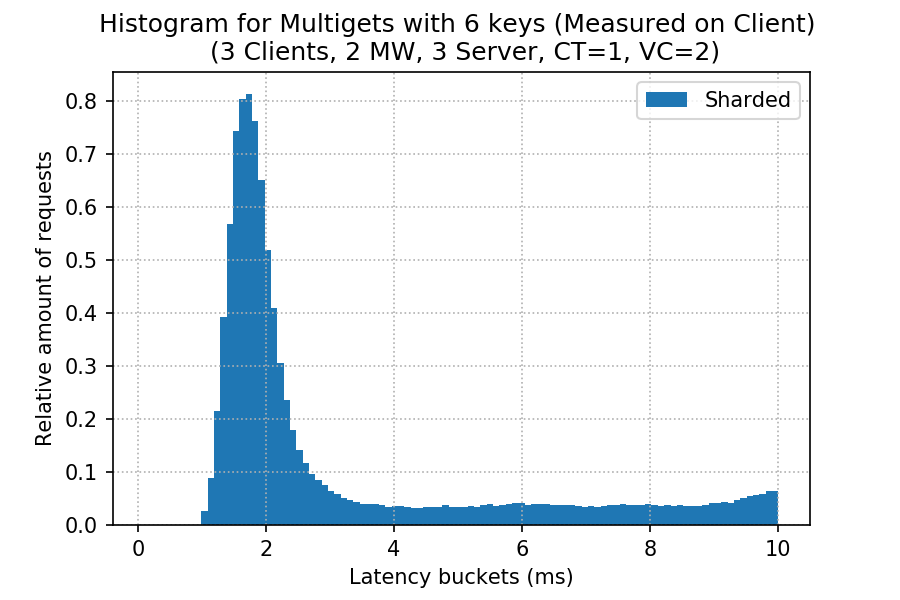
\includegraphics[width=\textwidth]{figures/4_GetsAndMultigets/mem_histogram_sharded_2018-11-22_18h12.png}
        \end{subfigure}
        \hfill
        \begin{subfigure}[b]{0.475\textwidth}  
            \centering 
            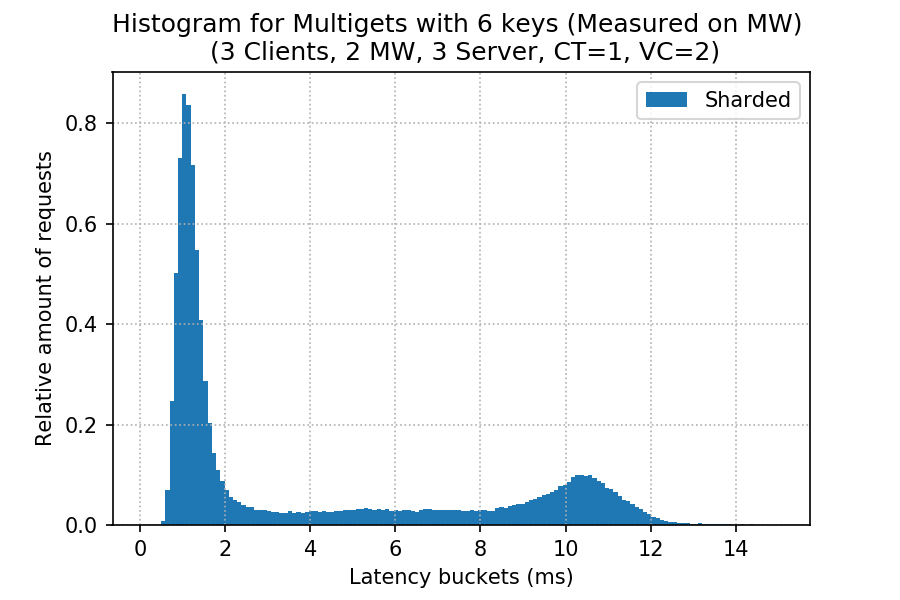
\includegraphics[width=\textwidth]{figures/4_GetsAndMultigets/mw_histogram_sharded_2018-11-22_18h12.png}
        \end{subfigure}
        \vskip\baselineskip
        \begin{subfigure}[b]{0.475\textwidth}   
            \centering 
            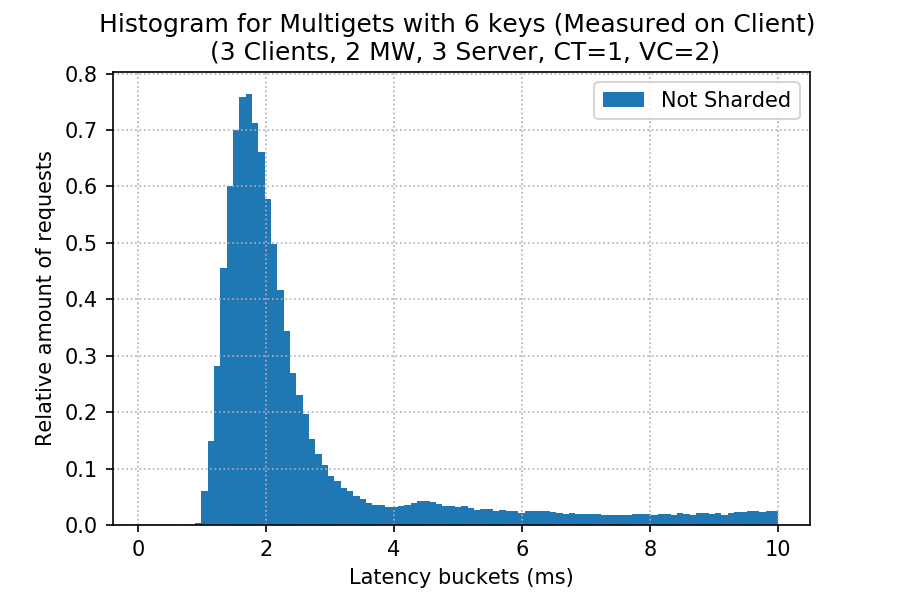
\includegraphics[width=\textwidth]{figures/4_GetsAndMultigets/mem_histogram_nonsharded_2018-11-22_18h12.png}
        \end{subfigure}
        \quad
        \begin{subfigure}[b]{0.475\textwidth}   
            \centering 
            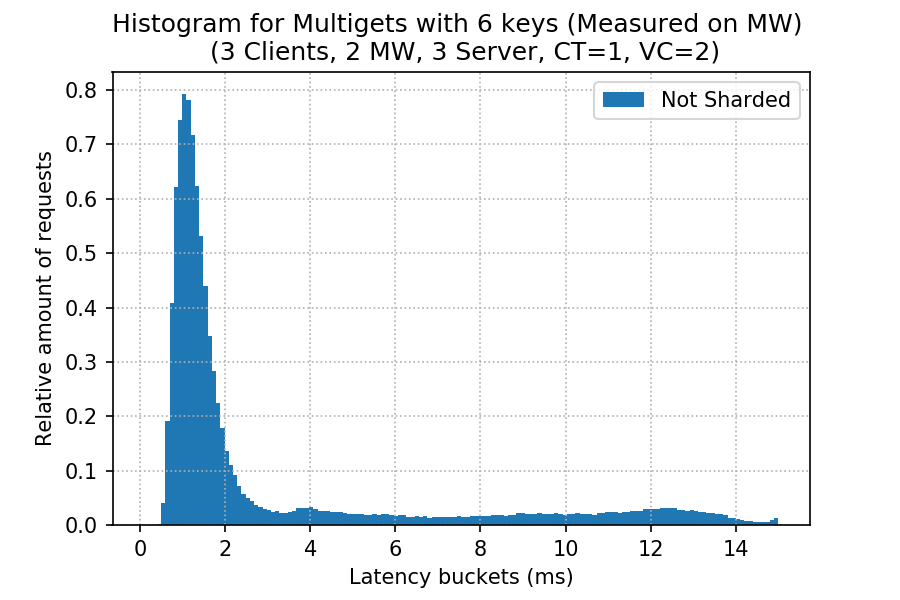
\includegraphics[width=\textwidth]{figures/4_GetsAndMultigets/mw_histogram_nonsharded_2018-11-22_18h12.png}
        \end{subfigure}
         \caption[]
        {\small Histograms of the response time distribution of sharded and non-sharded multigets measured on the client (left column) and on the middleware (right column). } 
        \label{histograms}
    \end{figure}
    
% explain
Generally we can say that the majority of requests are processed within 3ms for both the sharded and the non-sharded case. Also the histogram plots conform with the percentile plots. For the sharded-case we have 50\% of request being processed within 2ms, 75\% within 9ms, 90\% within 11ms and 99\% within 13ms. For the non-sharded case we have 50\% of request being processed within 2ms, 75\% within 4ms, 90\% within 15ms and 99\% within 15ms. In the sharded case, the 75th and 90th percentiles are significantly larger than in the non-sharded case, which is because in the sharded case we have a hill around 11ms, which will be explained later.

Comparing the client plots with the middleware plots, we see that the peak of the middleware plots is closer to  0ms than on the client plot. This is because of the network latency between the clients and middlewares which is not included in the middleware response time. We can also see that the distributions on the middleware are a little more narrow than on the clients. This is because the response time measured on clients captures a longer route of requests than the response time measured on the middlewares and thus we have more variability in the response time. Note that we had to cut the distributions measured on clients at 10ms because memtier did increase the bucket size from 0.1ms to 1ms after 10ms, which is too coarse grained. But essentially the continuation of the distributions can be seen in the middleware plots.

Comparing the sharded plots with the non-sharded plots, we can see that in the non-sharded case the distribution around the peak is more spread out than in the sharded case. This is because in the non-sharded case the response time of a request depends on the chosen server by the round-robin load balancer, which is not the same for every request, whereas in the sharded case, the response time is always determined by the slowest server and thus the response time of all requests is bound by this server, which leads to a more narrow distribution around the peak. Since the network latency between a middleware and a server is around 1ms for all servers, we only have one peak in the non-sharded case but I would expect multiple peaks if we had larger differences in latencies. 

What remains to be mention is the small hill around 10ms in the sharded case. I assume this is because of the bottleneck at the server which leads to congestion and thus to some requests having to wait longer than others to get processed. The hill almost disappeared in the non-sharded case, which might be because the probability for this delay at the server is smaller due to a request only involving one server and not all servers. This would support the hypothesis. 

\subsection{Summary}
%Compare the two modes with each other (for which multiget size is sharding preferred)
To conclude, non-sharding might be preferred over sharding because of a better average response time. This is because in the non-sharded case not all multigets are limited by the slowest server or largest latency to a server like in the sharded case. Also, sharding has an overhead of dividing multigets, combining responses and sending respectively receiving data from three instead of one server. The larger the service time differences between the servers and the network latency differences to the servers are, the bigger the average response time difference between the sharded and non-sharded case would be for the number of keys analyzed in this section.

\section{2K Analysis (90 pts)}
%% Intro
In this chapter we want to figure out the effect of different parameters on the response time and the throughput with a 2k analysis. \\
More specifically, we conduct a $2^k*r$ analysis with three factors ($k=3$) and with three repetitions ($r=3$). The analysis is done for two different workloads (read-only and write-only) and for two different response variables (throughput and response time), i.e. in total we conduct four $2^k*r$ analyses. \\
The three factors we consider are the number of memcached servers, the number of middlewares and the number of worker threads. Each factor can assume two levels ($-1$ and $1$), which represent a specific configuration as given in the following table:
\begin{center}
	\scriptsize{	
		\begin{table}[!ht]
			\centering
			\begin{tabulary}{\linewidth}{ | C | C | C | C | }
				\hline 	&	Number of servers (\textbf{A})	&	Number of middlewares (\textbf{B})	& Number of workers (\textbf{C})	\\
				\hline	-1	&	1	&	1	&	8	\\
				\hline	1	&	3	&	2	&	32	\\
				\hline 
			\end{tabulary}
		\end{table}
	}
\end{center}
To get the input data of the analysis we first need to run the experiments. We let each experiment run for 90s and each experiment is repeated 3 times.  The first and last 10 seconds of an experiment are part of the warm-up and cool-down phase and are thus ignored. The overview of the experiment parameters is shown in the following table:
\begin{center}
	\scriptsize{
		\begin{tabular}{|l|c|}
			\hline Number of servers                & 1 and 3                                     \\ 
			\hline Number of client machines        & 3                                           \\ 
			\hline Instances of memtier per machine & 1 (1 middleware) or 2 (2 middlewares) \\ 
			\hline Threads per memtier instance     & 2 (1 middleware) or 1 (2 middlewares)   \\
			\hline Virtual clients per thread       &  32                                     \\ 
			\hline Workload                         & Write-only and Read-only\\
			\hline Number of middlewares            & 1 and 2                                     \\
			\hline Worker threads per middleware    & 8 and 32                                    \\
			\hline Repetitions                      & 3                                  \\ 
			\hline 
		\end{tabular}
	} 
\end{center}

% additive or multiplicative model
The multiplicative model was chosen for all four analyses. It assumes that the effect of the factors, their interactions and the errors are multiplicative. The multiplicative model does explain our data very well because the unexplained variation of effects is less than $0.65\%$ in all analyses.
All we have to do in the multiplicative model in contrast to the additive one, is to take the log of the measurements. Then the calculations remain the same.  \\

% explain tables
Before doing the interpretation of the results of the analyses, we want to explain what has been done in the tables which can be found at the end of this section. Note that all computations are done as explained in chapter $18$ of the book "The Art of Computer Systems Performance Analysis" by Raj Jain\footnote{Raj Jain, The Art of Computer Systems Performance Analysis: Techniques for Experimental Design, Measurement, Simulation, and Modeling, April 1991, ISBN: 978-0471503361.}. 
First of all, the input data, which is the measured response for different configurations and repetitions, is colored in yellow. Note that we take the log because of the multiplicative model. 
The effect variables $q$ can be computed using the sign table method. The signs of the sign table are colored in red, while the effect variables are colored in green. The importance of a factor $j$ is computed as the proportion of total variance in the response that is explained by that factor. It can be computed as $SSj/SST$, where $SST$ (the Sum of Squares Total) is the total variance of the response $y$ and $SSj$ (the Sum of Squares due to factor $j$) is the portion of $SST$ that is explained by factor $j$.
The difference between the estimated and measured response values are called the experimental errors and are colored in purple. The Sum of Squared Errors (SSE) is used to estimate the variance of the errors and to compute the confidence intervals for the effects for which the t-value at $16$ ($=2^k(r-1)$) degrees of freedom and $90\%$ confidence was chosen. If $0$ is included in the confidence interval, the effect can be considered insignificant. \\


%% write only
$\bullet$ \textbf{Write-only workload:} The number of middlewares explains $73.5\%$ of the variation of effects on the throughput, which is by far the strongest effect. Then we have the number of servers with $14.7\%$ of variation of effects on the throughput but they have a negative effect. The number of workers explain $7.9\%$ of the variation of effects on the throughput and have a positive effect. \\
Those numbers make sense: In section \ref{section:BaselineWithMW} we saw that for the write-only workload going from 1 to 2 middlewares almost doubled the maximum achievable throughput because the net-thread bottleneck was relieved. Increasing the workers also increased the throughput because more requests can be processed in parallel, but not as significant as going from 1 to 2 middlewares. Increasing the number of servers has a negative effect on the throughput because of the replication that adds overhead to the system. \\
Almost all interactions-effects are either statistically insignificant or can be considered negligible, with the exception of the interaction-effect of the middlewares and the workers, which has $2.5\%$ of variation of effects. This is because increasing the number of middlewares also increases the number of workers. \\
The percentages of variation of throughput and response time are basically the same with small deviations, which is what we expect because of the interactive response time law. But for the response time, the sign of significant effects are opposite to the throughput because they relate inverse proportionally to each other. \\

%% read-only
$\bullet$ \textbf{Read-only workload:} For the read-only workload the variation of effects can be explained entirely by the number of servers. All other effects are statistically insignificant or negligible. \\
This is because of the outbound network bandwidth bottleneck at the servers. If we fix the number of servers, this bottleneck puts a hard limit on the maximum achievable throughput, which we can also compute as  (maximum bandwidth per server * \#servers)/ size of a Get response. Thus changing number of workers (8 or 32) or changing the number of middlewares (1 or 2) does not change anything regarding throughput under this bottleneck. But going from 1 to 3 servers increases throughput from 3k ops/s to almost 9k ops/s because we have three times more outbound network bandwidth at the servers in total. \\
The response time analysis also conforms to the throughput analysis and relates in the same way to it as explained for the write-only workload. 

%% insert tables
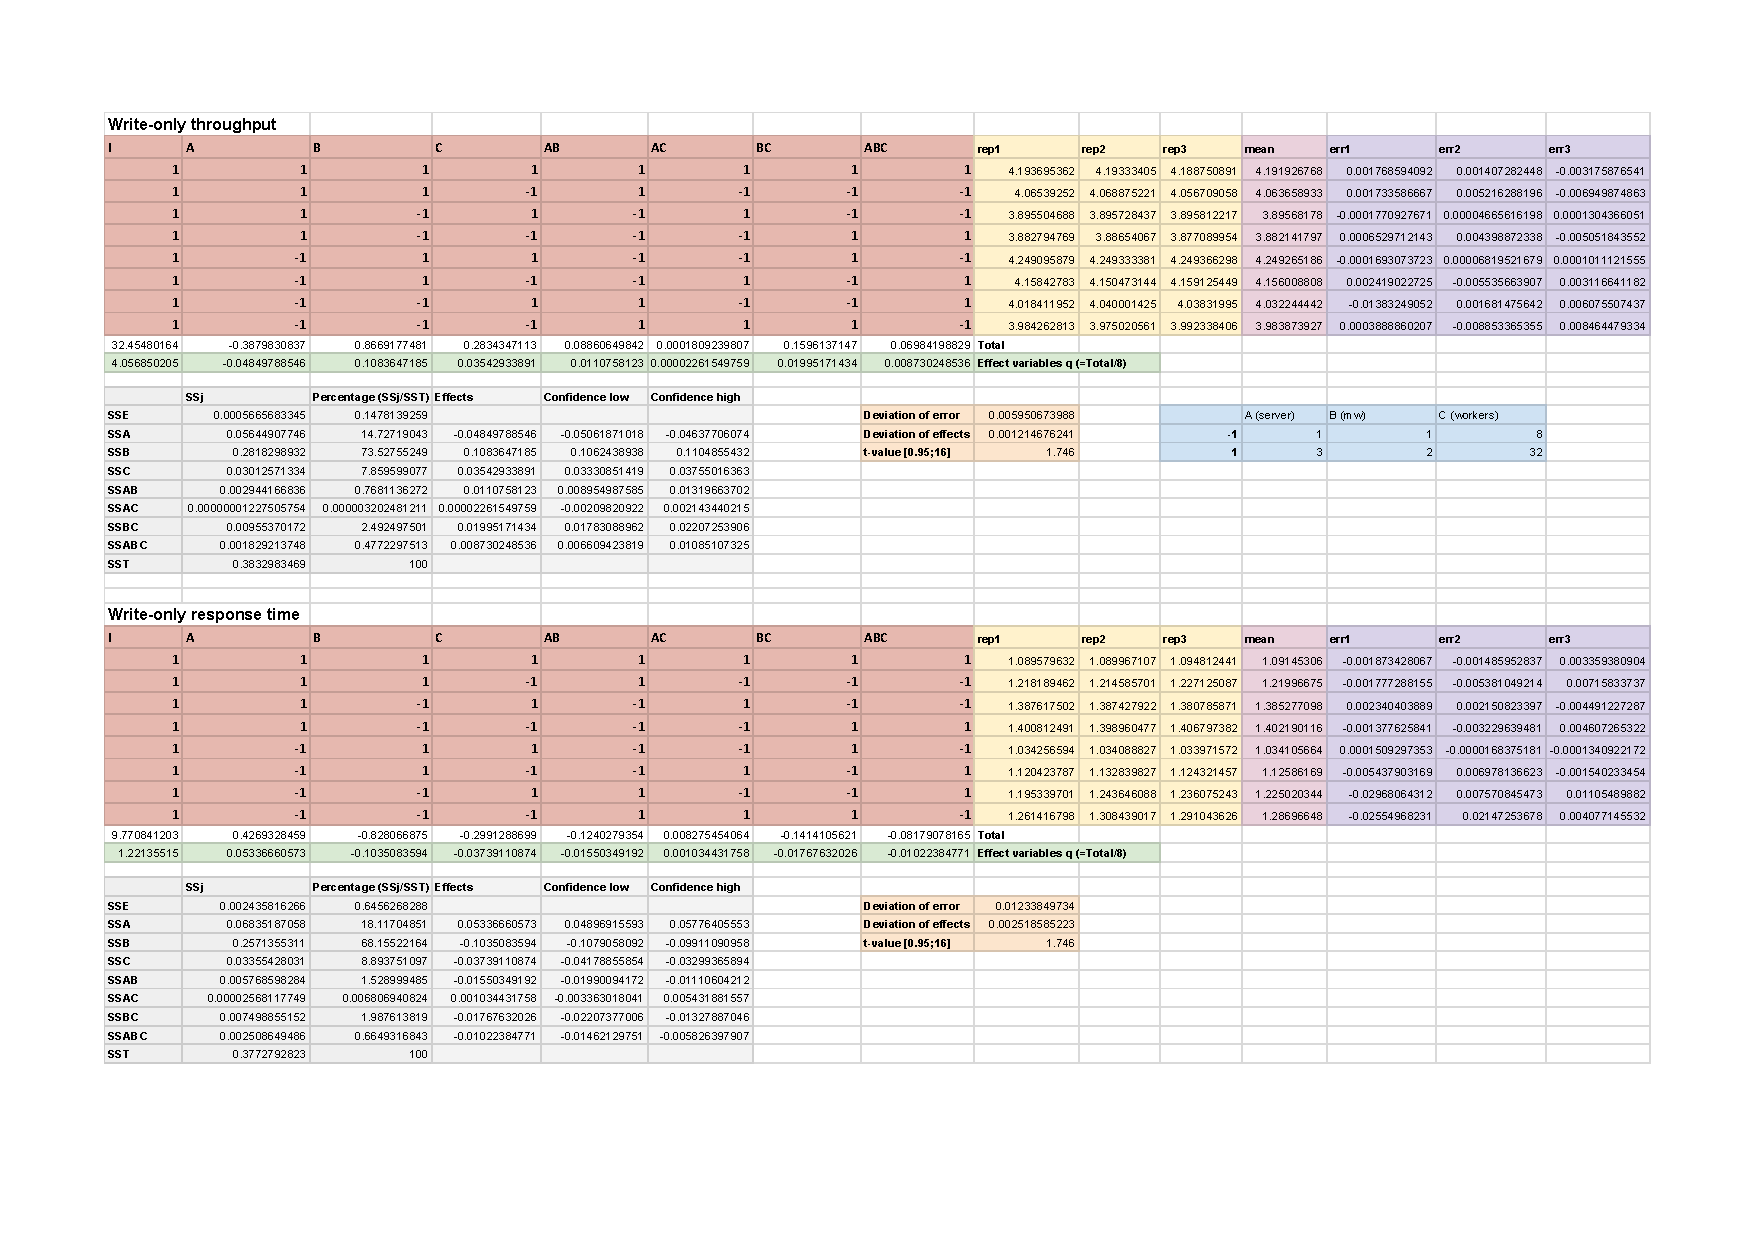
\includepdf[pages=-,scale=1,landscape=true]{figures/5_2kAnalysis/2kAnalysis_multiplicative_WO_2018-11-15_07h37.pdf}
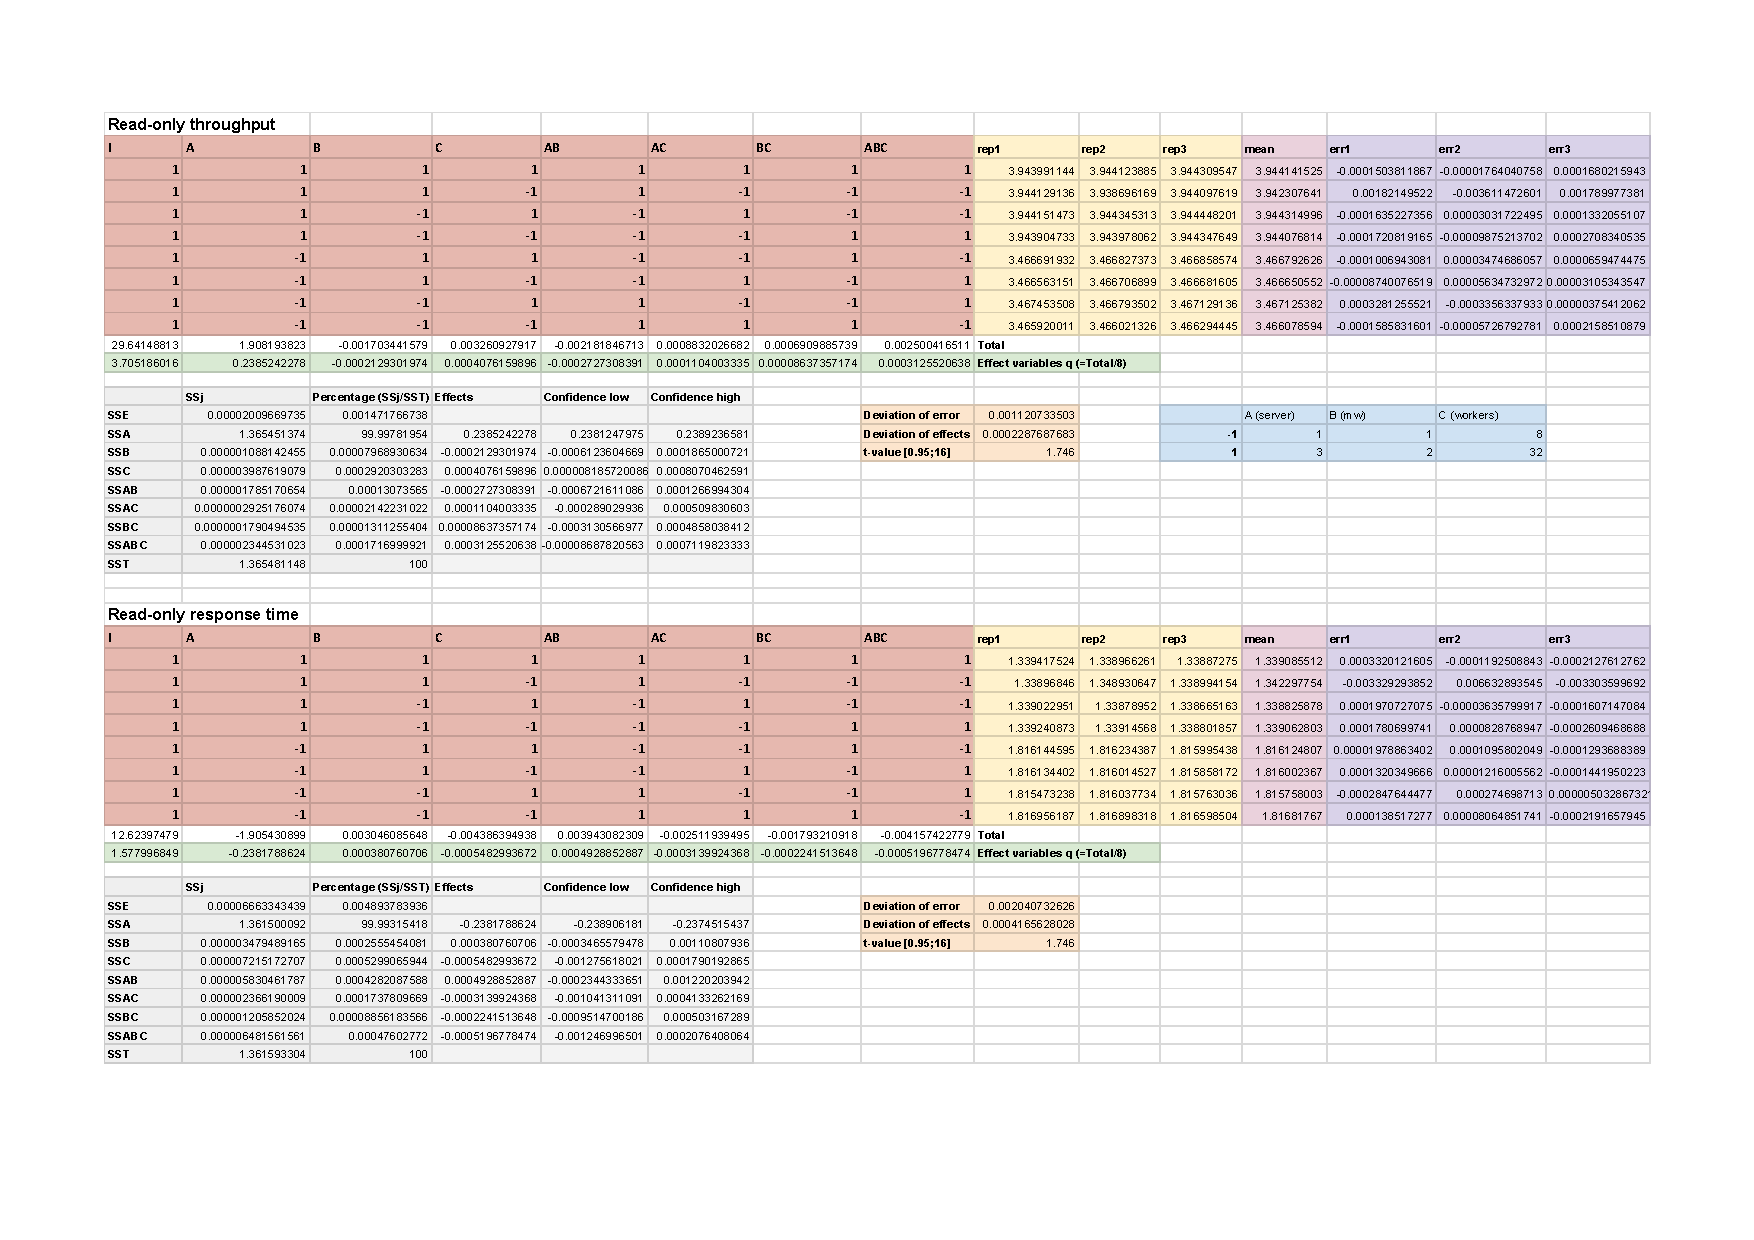
\includepdf[pages=-,scale=1,landscape=true]{figures/5_2kAnalysis/2kAnalysis_multiplicative_RO_2018-11-15_07h37.pdf}

\section{Queuing Model (90 pts)}
%% Intro
The goal of this section is to develop an analytical queuing model for each component of the system and for the system as a whole. We derive the performance characteristics that the model predicts and compare them with the results obtained in the experiments. We start with a naive model and progressively improve it to better fit our system. 

\subsection{M/M/1}
%% Explain model
In this subsection we build an M/M/1 model based on Section \ref{section:TpForWrites} (Throughput for Writes). 
First of all, we need to define the model boundaries: We choose the net-threads to be the entry point of the system, and the worker threads sending back a response to the clients mark the endpoint of the system. 
The single service of the M/M/1 model represents all the worker threads of the two middlewares together. Note that the service time also includes the memcached RTT because a service having finished serving a job corresponds in the real system to the event of a worker thread sending back a response to the client. The queue in front of the service represents the internal request queues of both middlewares together. 
This is a naive model and has several differences to the actual system which are discussed at the end of this subsection. \\

%% Input parameters of model
\textbf{Input parameters of the model:} %//
\begin{itemize}
\item[--] \textit{mean service rate }$\mu$: We are going to analyze each worker configuration separately. That's why for each worker configuration we choose the maximum observed throughput as an approximation of its mean service rate.
\item[--] \textit{mean arrival rate} $\lambda$: The mean arrival rate is computed as the throughput of the middleware for a specific client load and the analyzed worker configuration. Note that this can only be done because we are in a closed system. For the client load we choose 144 clients because we expect to observe an interesting change in behavior.
\end{itemize}

%% Make predictions based on model and input values
\textbf{Predictions based on the model and the input values:} First we list the metrics we want to predict and also the corresponding formulas. The formulas are derived from operational laws and can be seen in chapter 31 of the book "The Art of Computer Systems Performance Analysis" by Raj Jain\footnote{Raj Jain, The Art of Computer Systems Performance Analysis: Techniques for Experimental Design, Measurement, Simulation, and Modeling, April 1991, ISBN: 978-0471503361.}. We already include the formulas for the M/M/m model of the next subsection. Note that $\varrho$ is the probability of \textit{m} or more jobs in system: \\ $\varrho=[(mp)^m/(m!(1-p))]*p_0$ where $p_0$ is the probability of zero jobs in the system.
\begin{table}[H]
		\centering
	\begin{tabular}{|c|c|c|}
		\hline
		\multicolumn{1}{|c|}{Metric} & \multicolumn{1}{c|}{M/M/1} & \multicolumn{1}{c|}{M/M/m}\\ \hline
		Traffic load/Utilization $\rho$ & $\lambda/\mu$ & $\lambda/(m\mu)$ \\ \hline
		Mean num jobs in queue $E[n_q]$     & $ \rho^{2}/(1 - \rho)$& $\rho \varrho / (1 - \rho)$ \\ \hline
		Mean num jobs in service $E[n_s]$   & $\rho$ & $m \rho$\\ \hline
		Mean num jobs in system $E[n]$      & $\rho / (1-\rho)$ & $m\rho + \rho \varrho / (1 - \rho)$ \\ \hline
		Mean waiting time $E[w]$            & $\rho \frac{1/\mu}{(1 - \rho)}$ & $\varrho/ [m\mu(1 - \rho)]$\\ \hline
		Mean service time $E[s]$            & $1/\mu$ & $1/\mu$ \\ \hline
		Mean response time $E[r]$           & $ (1/\mu)/(1 - \rho)$ & $\frac{1}{\mu} (1 + \frac{\varrho}{m(1 - \rho)})$ \\ \hline
	\end{tabular}
	\label{}
\end{table}

%%Explain
Results are displayed in Table \ref{table:MM1}. 
First note that the traffic intensities $\rho$ are strictly smaller than $1$, thus the stability condition holds.
Utilization for 8, 16 and 32 workers is almost at 100\%, which matches the behaviour of the system in Section \ref{section:TpForWrites} because workers are the bottleneck and the system is fully saturated at 144 client load (see Figure \ref{full_write_tp}).
For 64 workers, the client load of 144 does not reach saturation yet because there are enough workers that process requests. The model correctly predicts the utilization decrease for 64 workers. 

The queue lengths are not accurately predicted, which might be because of the following reasons:
\begin{enumerate}
\item We have a fixed number of requests in the actual system because it is closed but in the model the queue length can increase even further because it corresponds to an open system. The model is not closed because it has a fixed arrival rate and there are no clients that wait for a response.
\item The actual system has two internal request queues instead of one queue.
\item Small changes in utilization around 100\% result in large changes in the queue length because we only have one very fast service. Reaching high utilization of a single fast service has a more negative impact on the queue length than if multiple slower services reach their limit. This implies that for lower utilization we should have more accurate predictions, which is indeed the case, as can be seen from the queue length and the queue waiting time for 64 workers. 
\end{enumerate}
The number of jobs in service is very under-estimated because the model has only one service which cannot process more than one job at a time and thus $E[n_s] \leq 1$. But in the actual system multiple workers can process jobs in parallel and thus we can have more than one job receiving service. This also leads to the number of jobs in system being under-estimated. \\
Total response times are not accurately predicted because the service time is very underestimated and the waiting time is also not accurate because of the same reason the queue length is not accurately predicted. 

\begin{table}[!ht]
	\begin{adjustbox}{center}
		\begin{tabulary}{\linewidth}{ C | C | C | C | c | C | C | C | C | }
			\cline{2-9}	&	\multicolumn{2}{| c |}{\textbf{8 workers}}	&	\multicolumn{2}{| c |}{\textbf{16 workers}}	&	\multicolumn{2}{| c |}{\textbf{32 workers}}	&	\multicolumn{2}{| c |}{\textbf{64 workers}}	\\
			\cline{2-9} &	predicted	&	measured	&	predicted	&	measured	&	predicted	&	measured	&	predicted	&	measured	\\
			\hline	\multicolumn{1}{| c |}{$\mu$ [req/s]}	    &-      &9249.94&-	&10891.57	&-	&13258.34	&-	&15670.26	\\
			\hline	\multicolumn{1}{| c |}{$\lambda$ [req/s]}	&-      &9025.93&-	&10716.8	&-	&13023.1	&-	&14519.22	\\
			\hline	\multicolumn{1}{| c |}{$\rho$}	            &0.9758	&-	    &0.984	&-	&0.9823	&-	&0.9265	&-	\\
			\hline	\multicolumn{1}{| c |}{$\mathbb{E}[n_q]$}	&39.32	&59.7	&60.33	&48.39	&54.38	&27.2	&11.69	&6.94	\\
			\hline	\multicolumn{1}{| c |}{$\mathbb{E}[n_s]$}	&0.98	&16	&0.98	&32	&0.98	&64	&0.93	&128	\\
			\hline	\multicolumn{1}{| c |}{$\mathbb{E}[n]$}	    &40.29	&75.7	&61.32	&80.39	&55.36	&91.2	&12.61	&134.94	\\
			\hline	\multicolumn{1}{| c |}{$\mathbb{E}[w]$ [ms]}&4.36	&13.6	&5.63	&9.78	&4.18	&5.12	&0.8	&0.84	\\
			\hline	\multicolumn{1}{| c |}{$\mathbb{E}[s]$ [ms]}&0.11	&1.77	&0.09	&2.99	&0.08	&4.91	&0.06	&7.19	\\
			\hline	\multicolumn{1}{| c |}{$\mathbb{E}[r]$ [ms]}&4.46	&15.37	&5.72	&12.77	&4.25	&10.03	&0.87	&8.03	\\
			\hline
		\end{tabulary}
	\end{adjustbox}	
	\caption{Predicted and measured metrics of the M/M/1 model for all worker configurations under the load of 144 clients.}
	\label{table:MM1}
\end{table}

%% Describe difference between model and actual system
To conclude, we can say that the model is too simple and cannot predict the experiment results very well because of the following differences to the actual system: In reality we have two internal request queues and not only one because we have two middlewares. The worker threads correspond to multiple services that run in parallel and not to a single sequential service. The model represents an open system because jobs arrive at a fixed arrival rate, and there is no flow of requests where finished jobs are again enqueued at the beginning. But the actual system is a closed one. Another difference is that memcached servers and workers are both in the same service instead of considered independently from each other. 

\subsection{M/M/m}
%% Explain model
In this subsection we build an M/M/m model based on Section \ref{section:TpForWrites}. The model consists of multiple services that process and dequeue jobs from a single queue in parallel. A service corresponds to a single worker thread and again the service time includes the memcached RTT. The queue in front of the services represents the internal request queues of both middlewares together like in the M/M/1 model. This is a more accurate model of our system than the M/M/1 model and should lead to better predictions. \\

%% Input parameters of model
\textbf{Input parameters of the model:} 
\begin{itemize}
\item[--] \textit{mean service rate} $\mu$: There are multiple ways to approximate the mean service rate. Either we take the inverse of the shortest observed service time where the service time consists of the worker preprocessing time, the memcached RTT and the worker postprocessing time. Or we take the maximum observed throughput and divide it by the number of services m. We have chosen the second approach because it lead to better predictions.
\item[--] \textit{mean arrival rate} $\lambda$: Average throughput of the middleware like in the M/M/1 model.
\item[--] \textit{number of services} $m$: We have as many services as total number of workers in the system i.e. m = worker configuration x 2.
\end{itemize}

\begin{table}[!ht]
	\begin{adjustbox}{center}
		\begin{tabulary}{\linewidth}{ C | C | C | C | c | C | C | C | C | }
			\cline{2-9}	&	\multicolumn{2}{| c |}{\textbf{8 workers}}	&	\multicolumn{2}{| c |}{\textbf{16 workers}}	&	\multicolumn{2}{| c |}{\textbf{32 workers}}	&	\multicolumn{2}{| c |}{\textbf{64 workers}}	\\
			\cline{2-9} &	predicted	&	measured	&	predicted	&	measured	&	predicted	&	measured	&	predicted	&	measured	\\
			\hline	\multicolumn{1}{| c |}{$\mu$ [req/s]}	    &-      &578.12&-	&340.36	&-	&207.16	&-	&122.42	\\
			\hline	\multicolumn{1}{| c |}{$\lambda$ [req/s]}	&-      &9025.93&-	&10716.8	&-	&13023.1	&-	&14519.22	\\
			\hline	\multicolumn{1}{| c |}{$\rho$}	            &0.9758	&-	    &0.984	&-	&0.9823	&-	&0.9265	&-	\\
			\hline	\multicolumn{1}{| c |}{$\mathbb{E}[n_q]$}	&35.85	&59.7	&54.87	&48.39	&46.35	&27.2	&3.73	&6.94	\\
			\hline	\multicolumn{1}{| c |}{$\mathbb{E}[n_s]$}	&15.61	&16	&31.49	&32	&62.86	&64	&118.6	&128	\\
			\hline	\multicolumn{1}{| c |}{$\mathbb{E}[n]$}	    &51.46	&75.7	&86.36	&80.39	&109.21	&91.2	&122.33	&134.94	\\
			\hline	\multicolumn{1}{| c |}{$\mathbb{E}[w]$ [ms]}&3.97	&13.6	&5.12	&9.78	&3.56	&5.12	&0.26	&0.84	\\
			\hline	\multicolumn{1}{| c |}{$\mathbb{E}[s]$ [ms]}&1.73	&1.77	&2.94	&2.99	&4.83	&4.91	&8.17	&7.19	\\
			\hline	\multicolumn{1}{| c |}{$\mathbb{E}[r]$ [ms]}&5.7	&15.37	&8.06	&12.77	&8.39	&10.03	&8.43	&8.03	\\
			\hline
		\end{tabulary}
	\end{adjustbox}	
	\caption{Predicted and measured metrics of the M/M/m model for all worker configurations under the load of 144 clients.}
	\label{table:MMm}
\end{table}

%% Make predictions based on model and input values
\textbf{Predictions based on model and input values:} 
Results are displayed in Table \ref{table:MMm}.
First note that the traffic intensities $\rho$ are strictly smaller than $1$, thus the stability condition holds.
The utilization predictions do match the reality pretty good as in the M/M/1 case. We now have higher service times, respectively lower service rates because we consider m services instead of a single one that models all the worker threads together. That's why the service time is now predicted more accurately than in the M/M/1 model where the service time was very short because of the extremely fast service, which lead to underestimated response times. 
Also the number of jobs in the service is predicted more accurately because it has no upper bound of 1 job anymore and thus also the total number of jobs is predicted more accurately. 
Note that still the response times are mostly predicted too optimistic since this is a more ideal model than our system because of the following: 
\begin{enumerate}
    \item If there are jobs in the queue and there are available workers, jobs will be dequeued and processed. But in our system this may not be the case, because a worker may be ready to dequeue but his queue is empty while the queue in the other middleware is not.
    \item Services operate at a fixed ideal service rate, which in a real system may vary. Also an open system has a fixed arrival rate which can be considered more ideal than a closed system that always has to wait for jobs to finish because if a job of a client is processed very slowly, the client cannot send another job during the processing time.
\end{enumerate}
To conclude, we can say that the M/M/m model is more accurate than the M/M/1 model but the predictions are still not perfect because of the mentioned differences to the real system. In both models the whole system is modeled as a black box. To be able to more accurately predict the behavior of the system, we need to model each component of the system which is done in the next subsection. 

%the following differences to the real system remain: The model still only has one queue instead of two separate queues for each middleware. The model represents an open system instead of a closed one. And finally we have queuing model for the system as a whole where the system

\subsection{Network of Queues}

In this subsection we build a network of queues based on Section \ref{section:BaselineWithMW} (Baseline with Middleware). This is an even more accurate model of our system and should lead to better predictions than the M/M/m model.
We consider both the one and two middleware configuration and analyze both read-only and write-only workloads. The number of worker threads is set to a constant. 

\subsubsection{System with one middleware}
%% Explain model
The model is shown in Figure \ref{NoQ_one_mw}. 
It is a closed queuing network, where jobs keep circulating from one queue to the next, i.e. we have a fixed number of jobs which we set equal to the number of clients. 
The network is modeled as a delay center. Delay centers have no queuing and the service time is independent of the load. The network delays can be computed from the measured ping times. \\
The memtier clients are modeled as a delay center because their queuing time is negligible and we adjust their service time to handle numerical instabilities. We only need a single delay center because the network delay between the clients and the middleware is roughly the same for all clients. \\
The net-thread is simulated with an M/M/1 model. It consists of one service because we have one net-thread and the queue represents the Java Selector in front of the net-thread which enqueues arriving requests from the clients. The service time is computed from the difference of timestamps when the net-thread reads a request and when it enqueues it. \\
The workers and the internal request queue is simulated with an M/M/m model where m is the number of workers. The service time includes the worker preprocessing time, the memcached RTT and the worker postprocessing time. We include the memcached servers in this component because of the Single-Resource Possession condition by Denning and Buzen (1978)\footnote{The Art of Computer Systems Performance Analysis by Raj Jain (chapter 32.2).} which states that a job may not be present at two or more devices at the same time.  If memcached servers were modeled as another component, then as soon as a worker sends a job to a memcached server it would take another job from its queue instead of waiting for the response of the memcached server. This would not model the behavior of our system. 

The model is implemented using the \textit{Octave} programming language and the \textit{queuing} package\footnote{Version 1.2.6 downloaded on \url{https://www.moreno.marzolla.name/software/queueing/}}.
Since we use load-dependent service centers (for the workers), we cannot use the basic MVA algorithm because they cannot be modeled using operational laws\footnote{Exercise session slides on network of queues (page 20).}. In this case we have to use the extended MVA algorithm, which is implemented in the mentioned queuing package of Octave.

\begin{figure}[!ht]
    \centering
	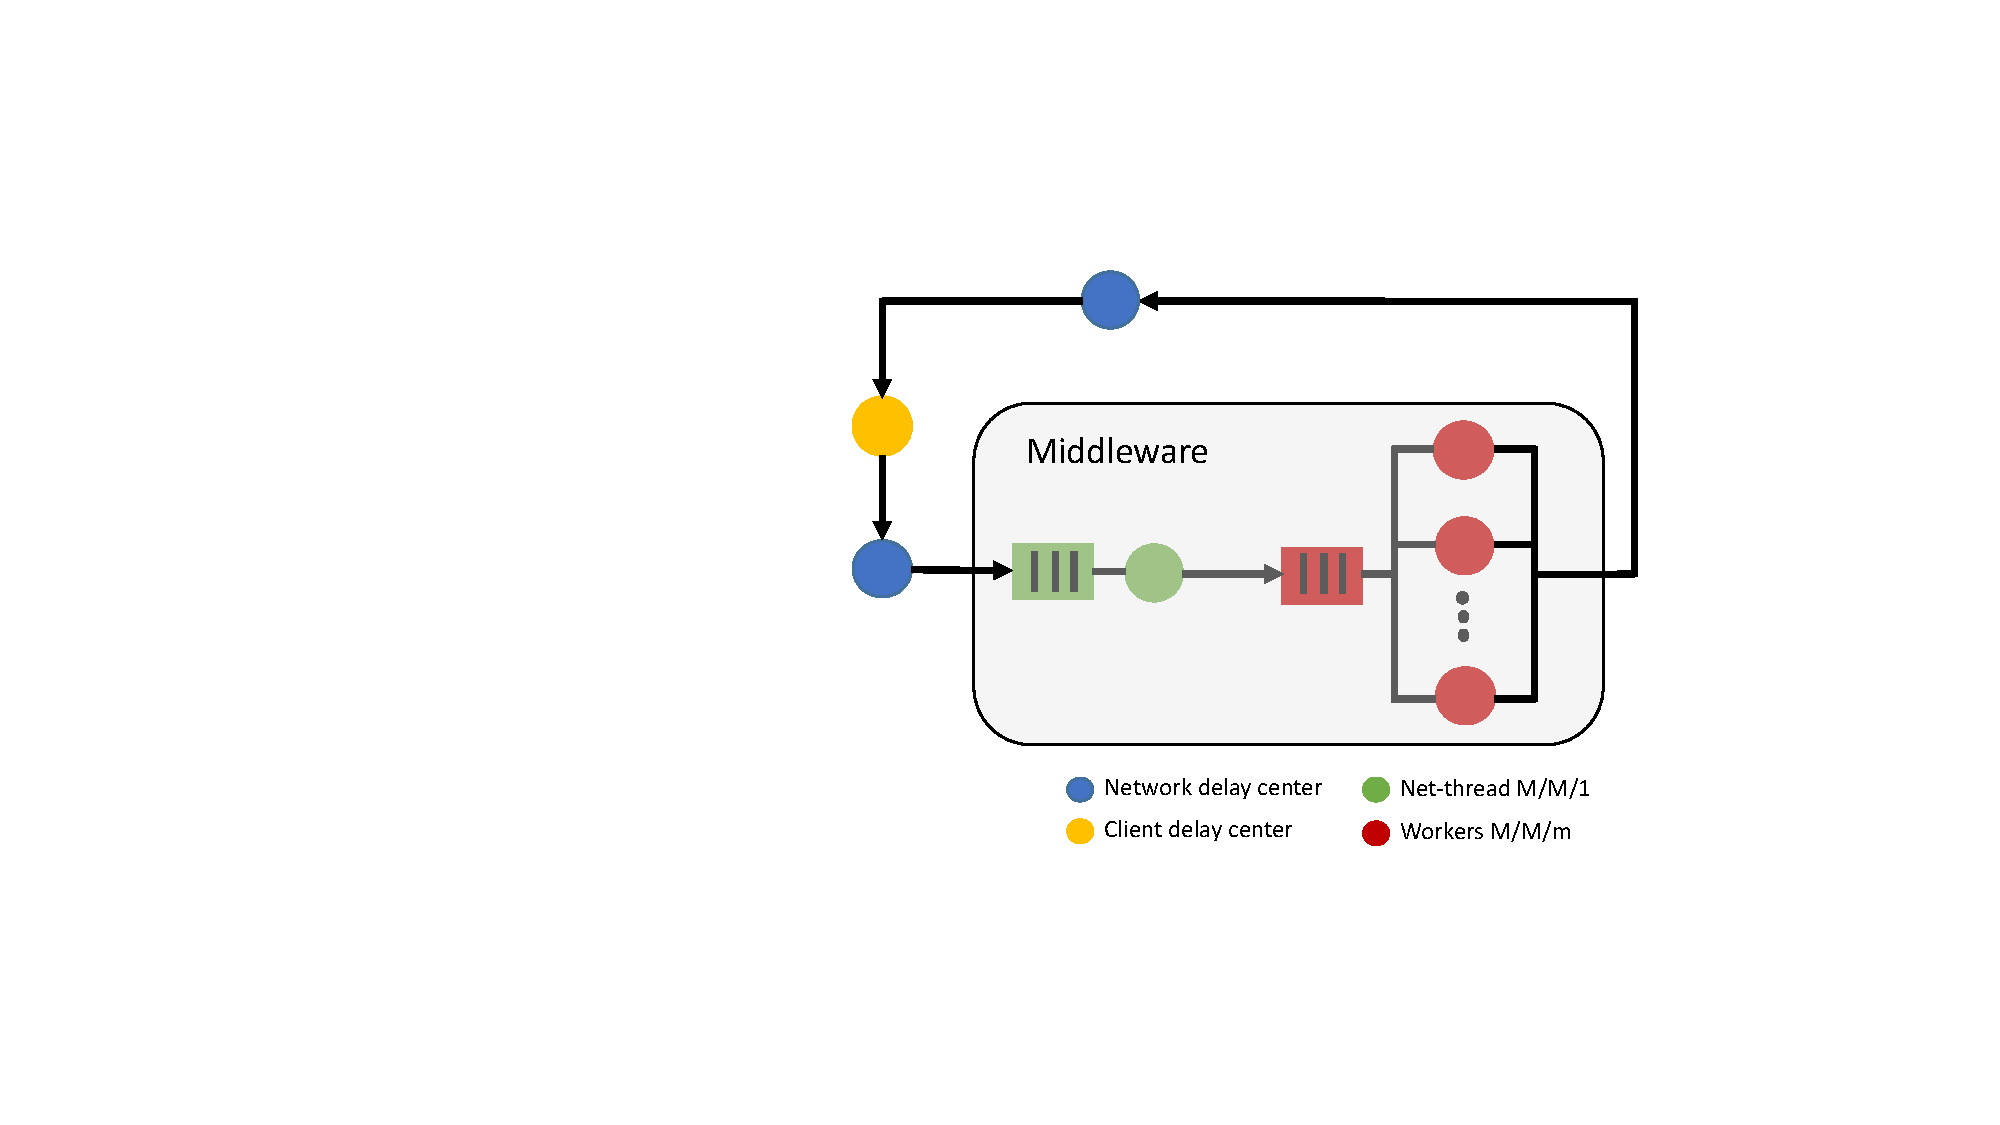
\includegraphics[scale=0.6]{figures/6_NoQ/NoQ_figure_one_mw.pdf}
	\caption{Network of queues model for one middleware case.}
	\label{NoQ_one_mw}
\end{figure}

%% Input parameters of model
The \textbf{input parameters} of the model are: \\
- worker service time and number of workers \\
- net-thread service time \\
- delays of the delay centers \\
- number of jobs circulating (= number of clients) \\
- visit ratios \\

%% Present and explain the predictions
Predicted metrics (from the output of Octave) and measured metrics for 8 workers and 48 client-load are shown in Table \ref{table:noq_1midd}. 
The predictions for the system throughput and the response time of the middleware are quite accurate. The predictions for the length of the internal request queue are also reasonably good. 
In contrast to the previous models, a network of queues allows us to do a bottleneck analysis. For the read-only workload, the bottleneck in our system of Section \ref{sec:baselineWithMWOne} was the memcached server respectively its outbound network bandwidth. This is correctly predicted by the model since $U_{workers} > U_{netthread}$ and based on our model $U_{workers}$ includes the memcached server. For the write-only workload, the bottleneck in our system (for 8 worker threads) were the worker threads, which is also correctly predicted as $U_{workers} > U_{netthread}$. The bottlenecks are at $100\%$ utilization which conforms to our system which is also saturated at 48 client-load with 8 worker threads for both read-only and write-only workloads.

If we compare read-only and write-only net-thread utilization, we see that the net-thread utilization for write-only is 5x higher than for read-only. This is because the SET requests are bigger and thus the net-thread needs to read more data in contrast to the GET requests which just contain a key. 

Another interesting point to mention is that if we do the write-only workload analysis for 64 workers, we have $58.11\%$ utilization for the net-thread and $26.65\%$ for the workers. Thus the model predicts that the bottleneck is on the net-thread and not on the worker threads anymore which exactly corresponds to the bottleneck analysis done in Section \ref{sec:baselineWithMWOne} as for higher number of workers the worker bottleneck is removed.

\begin{table}[!ht]
	\begin{adjustbox}{center}
		\begin{tabulary}{\linewidth}{ C | C | C | C | C | }
			\cline{2-5}	&	\multicolumn{2}{| c |}{\textbf{read-only}}	&	\multicolumn{2}{| c |}{\textbf{write-only}}	\\
			\cline{2-5} &	predicted	&	measured	&	predicted	&	measured	\\
			\hline	\multicolumn{1}{| c |}{throughput $X$ [req/s]}		&	2964.4	&	2938.08	&	7255.6	&	7112.42	\\
			\hline	\multicolumn{1}{| c |}{response time $R_{mw}$ [ms]}		&	15.26	&	15.4	&	5.59	&	5.74	\\
			\hline	\multicolumn{1}{| c |}{queue length $Q_{workers}$}				&	45.16	&	34.31	&	40.17	&	32.51	\\
			\hline	\multicolumn{1}{| c |}{utilization $U_{netthread}$ [\%]}	&	6.28	&	-		&	30.02	&	-	\\
			\hline	\multicolumn{1}{| c |}{utilization $U_{workers}$ [\%]}	&	100	&	-		&	100	&	-	\\
			\hline 
		\end{tabulary}
	\end{adjustbox}	
	\caption{\textit{Network of Queues for 8 workers and 48 client-load (one middleware)}.}
	\label{table:noq_1midd}
\end{table}

\subsubsection{System with two middlewares}
%% Explain model
The model is shown in Figure \ref{NoQ_two_mws}. 
Essentially everything is the same as in the one middleware case, but now the middleware part is duplicated i.e. the net-thread component is duplicated and also the worker thread component is duplicated. The traffic is split equally at the client among both net-threads.

\begin{figure}[!ht]
    \centering
	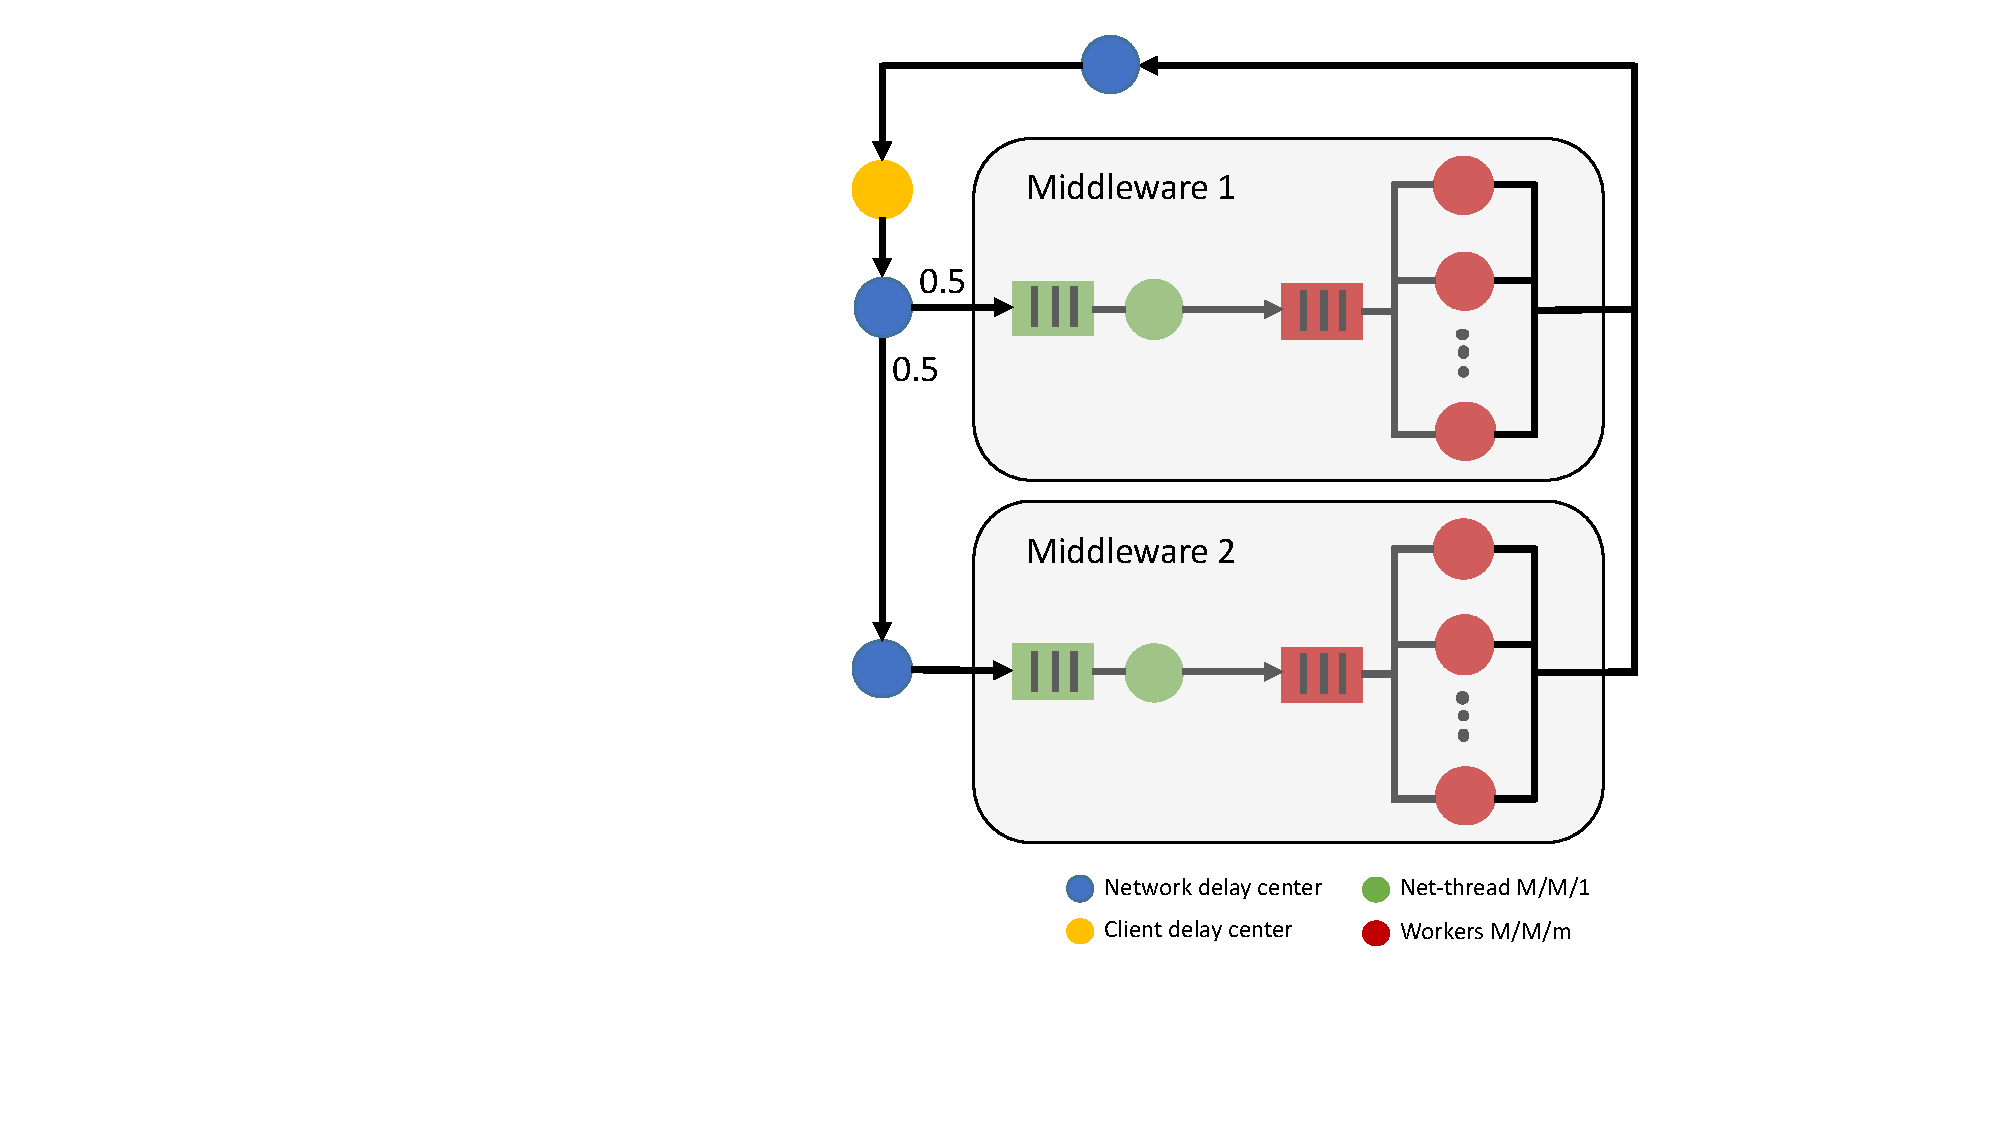
\includegraphics[scale=0.6]{figures/6_NoQ/NoQ_figure_two_mws.pdf}
	\caption{Network of queues model for two middlewares case.}
	\label{NoQ_two_mws}
\end{figure}

%% Present and explain the predictions
Predicted metrics (from the output of Octave) and measured metrics for 8 workers and 48 client-load are shown in Table \ref{table:noq_2midd}. 
Again the model predicts the throughput and response time of the middleware quite accurately. The queue length is predicted around 10 elements too high for both type of workloads. \\
For the read-only workload the predicted bottleneck are the worker threads because $U_{workers} > U_{netthread}$. This conforms to our bottleneck analysis in Section \ref{sec:baselineWithMWTwo} where the memcached server is the bottleneck, because again the servers are part of the M/M/m component representing the worker threads. 
For the write-only workload, the predicted bottleneck are also the worker threads for the same reason, which conforms to our bottleneck analysis in Section \ref{sec:baselineWithMWTwo} where the worker threads are the bottleneck. The bottlenecks are almost at $100\%$ utilization, which conforms to our system which is also saturated at 48 client-load with 8 worker threads for both read-only and write-only workloads.\\

If we compare the one middleware model predictions with the two middlewares model predictions, we see that especially for the write-only workload the utilization of the net-thread is significantly reduced going from one to two middlewares. 
This is because the two net-threads share the same load and we have less congestion in front of the Java Selector objects for the two middlewares configuration. 
\begin{table}[!ht]
	\begin{adjustbox}{center}
		\begin{tabulary}{\linewidth}{ C | C | C | C | C | }
			\cline{2-5}	&	\multicolumn{2}{| c |}{\textbf{read-only}}	&	\multicolumn{2}{| c |}{\textbf{write-only}}	\\
			\cline{2-5} &	predicted	&	measured	&	predicted	&	measured	\\
			\hline	\multicolumn{1}{| c |}{throughput $X$ [req/s]}		&	2869.2	&	2944.13	&	9184.1	&	9406.65	\\
			\hline	\multicolumn{1}{| c |}{response time $R_{mw}$ [ms]}		&	15.66	&	15.32	&	4.27	&	4.21	\\
			\hline	\multicolumn{1}{| c |}{queue length $Q_{workers}$}				&	22.44	&	11.63	&	19.47	&	10.67	\\
			\hline	\multicolumn{1}{| c |}{utilization $U_{netthread}$ [\%]}	&	2.06	&	-		&	13.98	&	-	\\
			\hline	\multicolumn{1}{| c |}{utilization $U_{workers}$ [\%]}	&	97.24	&	-		&	96.68	&	-	\\
			\hline 
		\end{tabulary}
	\end{adjustbox}	
	\caption{\textit{Network of Queues for 8 workers and 48 client-load (two middlewares)}.}
	\label{table:noq_2midd}
\end{table}

%% Conclusion
To conclude, we can say that the network of queues model provides accurate predictions of our system. But also network of queues have their limitations, and for example do not allow us to model the memcached servers and workers separately from each other. 

\end{document}
